\chapter{痛觉} \label{chap:chap20}
根据国际疼痛研究协会的说法,疼痛是一种与实际或潜在的组织损伤相关的不愉快的感觉和情绪体验,或者用这种损伤来描述。 
刺痛、灼痛、疼痛、刺痛和酸痛是所有感觉形态中最独特的。 
与其他体感方式(触觉、压力和位置感)一样,疼痛具有重要的保护功能,提醒我们注意需要逃避或治疗的伤害。 
在出生时对疼痛不敏感的儿童中,严重的伤害往往被忽视,并可能导致永久性组织损伤。 
然而,疼痛与其他体感方式或视觉、听觉和嗅觉不同,因为它具有紧迫和原始的性质,具有强大的情感成分。


对疼痛的感知是主观的,受许多因素的影响。 
相同的感官刺激可以在不同条件下引起同一个人的截然不同的反应。 
例如,许多受伤的士兵在离开战场之前不会感到疼痛; 
受伤的运动员通常直到比赛结束才意识到疼痛。 
简而言之,没有纯粹的“痛苦”刺激,即总是会引起所有人对疼痛的感知的感官刺激。 
疼痛感知的可变性是我们在前面几章中遇到的原则的另一个例子:
疼痛不是感觉事件的直接表达,而是大脑中各种神经信号精心处理的产物。


当经历疼痛时,它可能是急性的、持续的,或者在极端情况下是慢性的。 
持续性疼痛是许多临床病症的特征,通常是患者就医的原因。 
相比之下,慢性疼痛似乎没有任何用处; 
只会让患者痛苦不堪。 
疼痛的高度个体化和主观性是导致其难以客观定义和临床治疗的因素之一。


在本章中,我们将讨论构成正常人疼痛感知基础的神经过程,并解释临床上遇到的一些异常疼痛状态的起源。


\section{有害损伤激活温度、机械和多模式伤害感受器}
周围的许多器官,包括皮肤和皮下结构,如关节和肌肉,都具有专门的感觉感受器,这些感受器会被伤害性侮辱激活。 
与用于轻触和压力的专门体感感受器不同,这些伤害感受器中的大多数只是初级感觉神经元的游离神经末梢。 
伤害感受器主要分为三类:热感受器、机械感受器和多模式伤害感受器,还有更神秘的第四类,称为无声伤害感受器。


热伤害感受器被极端温度激活,通常高于 45°C (115°F) 或低于 5°C (41°F)。 
它们包括小直径的外围末端,以 5 至 30 m/s 的速度传导动作电位的薄髓鞘 Aδ 轴突和以小于 1.0 m/s 的速度传导的无髓鞘 C 纤维轴突(图\ref{fig:20_1} A)。 
施加在皮肤上的强烈压力可以最佳地激活机械伤害感受器;
它们也是有髓鞘的 Aδ 轴突的末端。
多模式伤害感受器可以被高强度的机械、化学或热(热和冷)刺激激活。
此类伤害感受器主要由无髓鞘 C 纤维组成(图 \ref{fig:20_1}A)。

\begin{figure}[htbp]
	\centering
	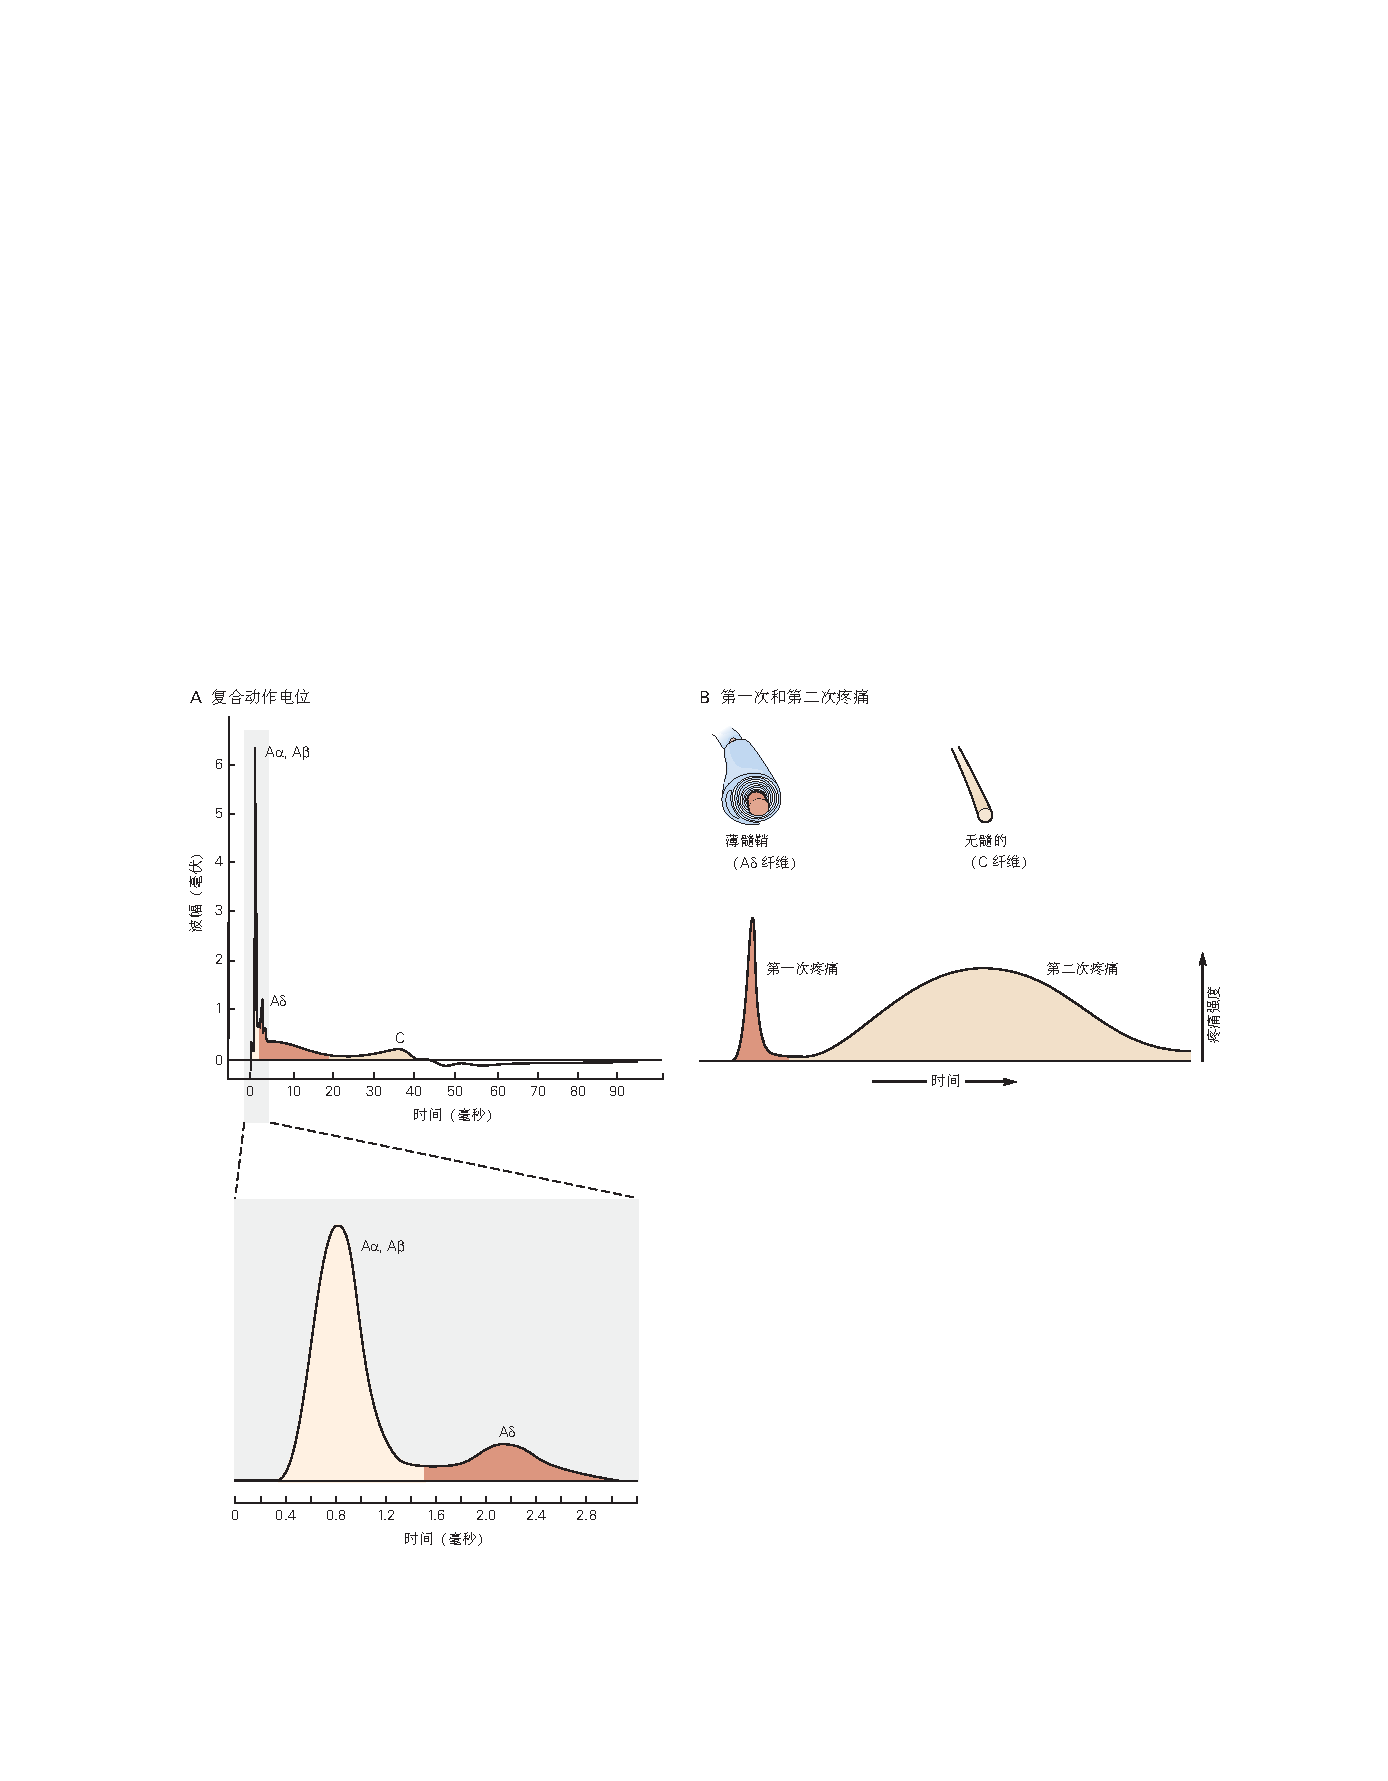
\includegraphics[width=0.7\linewidth]{chap20/fig_20_1}
	\caption{不同类别的伤害感受纤维中动作电位的传播。 
		A. 传导动作电位的速度是每根纤维横截面直径的函数。 
		图中的波峰按等待时间的字母顺序标记。 
		第一个峰值及其细分是有髓 A 纤维的电活动总和。 
		延迟(缓慢传导)偏转代表无髓鞘 C 纤维的总动作电位。 
		A 纤维的复合动作电位显示在更快的时基上,以描述几种纤维动作电位的总和。 (经许可改编自 Perl 2007。版权所有 © 2007 Springer Nature。) 
		B. 第一次和第二次疼痛分别由 A delta 和 C 纤维传递。 (经许可改编自 Fields 1987。)}
	\label{fig:20_1}
\end{figure}


这三类伤害感受器广泛分布于皮肤和深层组织中,并且经常被共同激活。
当锤子敲击您的拇指时,您最初会感到剧烈疼痛(“第一次疼痛”),然后是更长时间的疼痛,有时甚至是灼痛(“第二次疼痛”)(图 \ref{fig:20_1}B)。
快速锐痛是由 Aδ 纤维传输的,该纤维携带来自受损的热和机械伤害感受器的信息。
缓慢的钝痛是由 C 纤维传递的,C 纤维传递来自多模式伤害感受器的信号。


在内脏中发现了沉默的伤害感受器。 
这类受体通常不会被伤害性刺激激活; 
相反,炎症和各种化学试剂会显着降低它们的放电阈值。
它们的激活被认为有助于继发性痛觉过敏和中枢敏化的出现,这是慢性疼痛的两个显着特征。


有害刺激使传入轴突的裸露神经末梢去极化并产生向中央传播的动作电位。 
这是如何实现的? 
伤害感受器的膜包含将伤害性刺激的热能、机械能或化学能转化为去极化电位的受体。 
其中一种蛋白质是所谓的瞬时受体电位 (TRP) 离子通道大家族的成员。 
这种受体通道 TRPV1 由伤害性神经元选择性表达,并介导辣椒素、辣椒和许多其他刺激性化学物质的活性成分的疼痛产生作用。 
TRPV1 通道也会被有害热刺激激活,激活阈值约为 45°C,该温度会引发热痛。 
重要的是,TRPV1 介导的膜电流因 pH 值降低而增强,pH 值是炎症化学环境的一个特征。


TRP 通道家族的其他受体通道由伤害感受器表达,是对从寒冷到高温的广泛温度感知的基础。 
特别感兴趣的是 TRPM8,它是一种薄荷醇反应和冷敏感通道,可能介导许多化疗药物(如奥沙利铂)产生的极度冷超敏反应。 
TRPA1 对各种刺激物有反应,从芥末油到大蒜,甚至是空气污染物(图 \ref{fig:20_2})。 最近,描述了一个机械换能器系列(Piezo1 和 Piezo2)(第 \ref{chap:chap18} 章)。 
这些通道可能是机械超敏反应的重要贡献者,机械超敏反应是许多慢性疼痛病症的一个突出特征。


\begin{figure}[htbp]
	\centering
	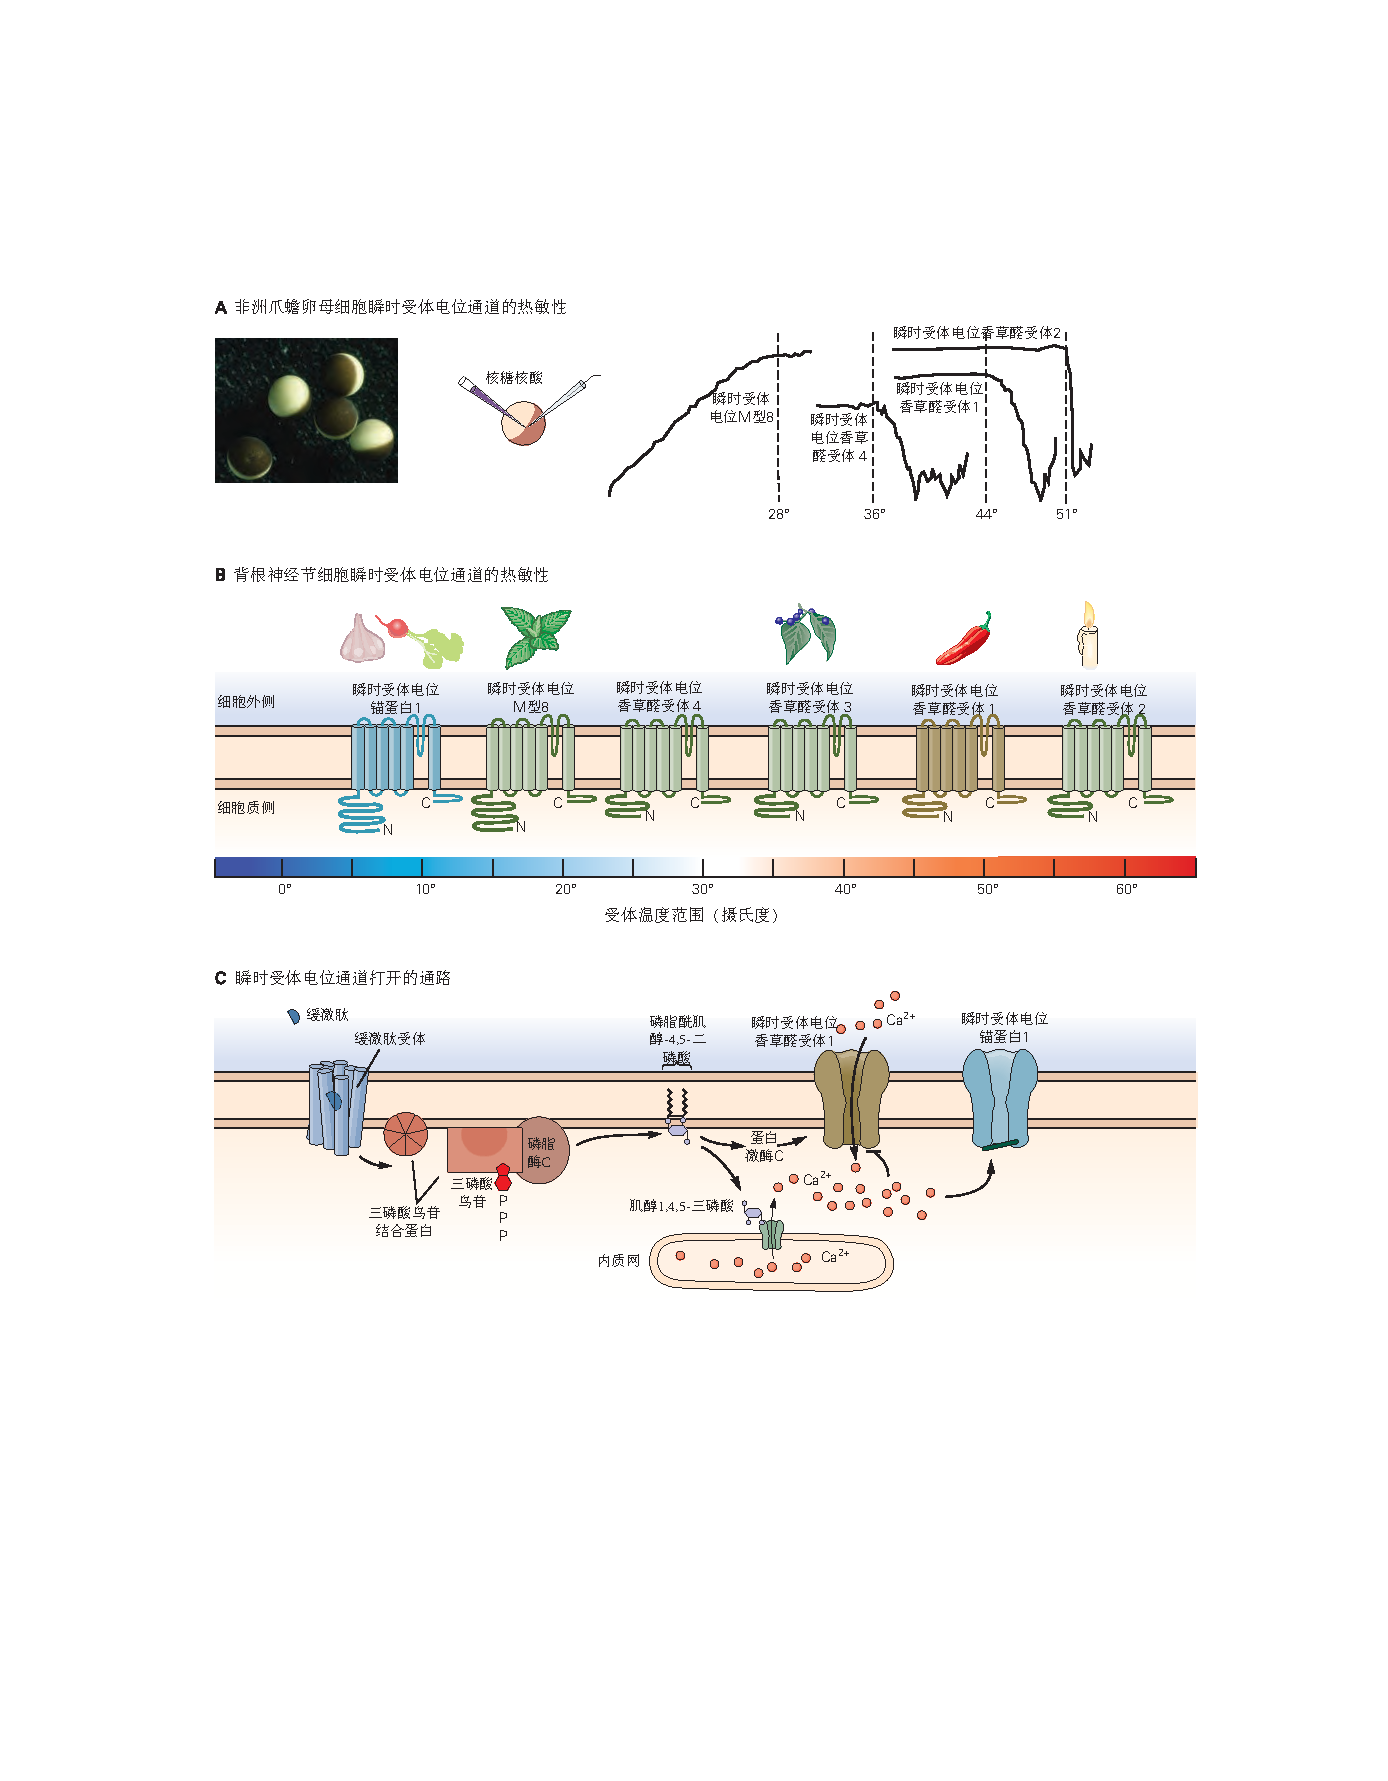
\includegraphics[width=0.7\linewidth]{chap20/fig_20_2}
	\caption{伤害性神经元中的瞬时受体电位离子通道。 
		A. 注射了 mRNA 编码瞬时受体电位 (TRP) 通道的非洲爪蟾卵母细胞的记录揭示了通道的热敏感性。 
		特定 TRP 通道被激活的温度(摄氏度)由记录的向下偏转显示。 (左图经许可转载自 Erwin Siegel 1987;右图经许可转载自 Tominaga 和 Caterina 2004。)
		B. 背根神经节神经元表达的不同 TRP 通道的温度响应曲线。 (经许可改编自 Jordt、McKemy 和 Julius 2003;Dhaka、Viswanath 和 Patapoutian 2006。)
		C. Bradykinin (BK) 与初级传入神经元表面的 G 蛋白偶联受体结合以激活磷脂酶 C (PLC) ),导致膜磷脂酰肌醇二磷酸 (PIP2) 的水解,肌醇 1,4,5-三磷酸 (IP3) 的产生,以及细胞内储存的 Ca2+ 的释放。 
		蛋白激酶 C (PKC) 的激活调节 TRP 通道活性。 
		TRPV1 通道被敏化,导致通道打开和 Ca2+ 流入。 (资料来源:Bautista 等人,2006 年。)}
	\label{fig:20_2}
\end{figure}

除了这个 TRP 通道群之外,感觉神经元还表达参与外周刺激转导的许多其他受体和离子通道。 
伤害感受器选择性地表达许多不同的电压门控 Na2+ 通道,这些通道是局部麻醉剂的目标,可以有效地阻止疼痛。 
(想想可以完全消除牙痛的牙医。)伤害感受器表达对河豚毒素 (TTX) 敏感或有抵抗力的 Na2+ 通道。 
一种类型的 TTX 敏感通道 Nav1.7 是人类感知疼痛的关键分子机制,正如在相应 SCN9A 基因中具有功能丧失突变的罕见个体中所揭示的那样。 
这些人对疼痛不敏感,但在其他方面都很健康,对触觉、温度、本体感觉、挠痒痒和压力表现出正常的感觉反应。 
SCN9A 基因中的第二类突变导致伤害感受器过度兴奋; 具有这些突变的个体表现出一种称为红斑性肢痛症的遗传病症,其中四肢有剧烈、持续的灼痛,并伴有极度发红(血管扩张)。 
由于 Nav1.7 与许多其他电压门控 Na+ 通道不同,它不存在于中枢神经系统中,因此制药公司正在开发拮抗剂,有望提供一种调节疼痛过程的新方法,而不会出现全身给药可能产生的不良副作用 利多卡因,可阻断电压门控 Na+ 通道的所有亚型。


伤害感受器还表达一种离子型嘌呤能受体 PTX3,该受体在组织损伤后由外周细胞释放的三磷酸腺苷 (ATP) 激活。 
此外,它们还表达 Mas 相关 G 蛋白偶联受体 (Mrg) 家族的成员,该家族可被肽配体激活并用于使伤害感受器对其局部环境中释放的其他化学物质敏感(见图\ref{fig:20_7})。 
这些无髓鞘传入神经的子集还包括对各种引起瘙痒的物质(包括致痒剂组胺和氯喹)有反应的受体通道。 
因此,这些受体和通道是开发选择性药物的有吸引力的目标,这些药物对感觉神经元有反应,对疼痛和瘙痒刺激有反应。


\begin{figure}[htbp]
	\centering
	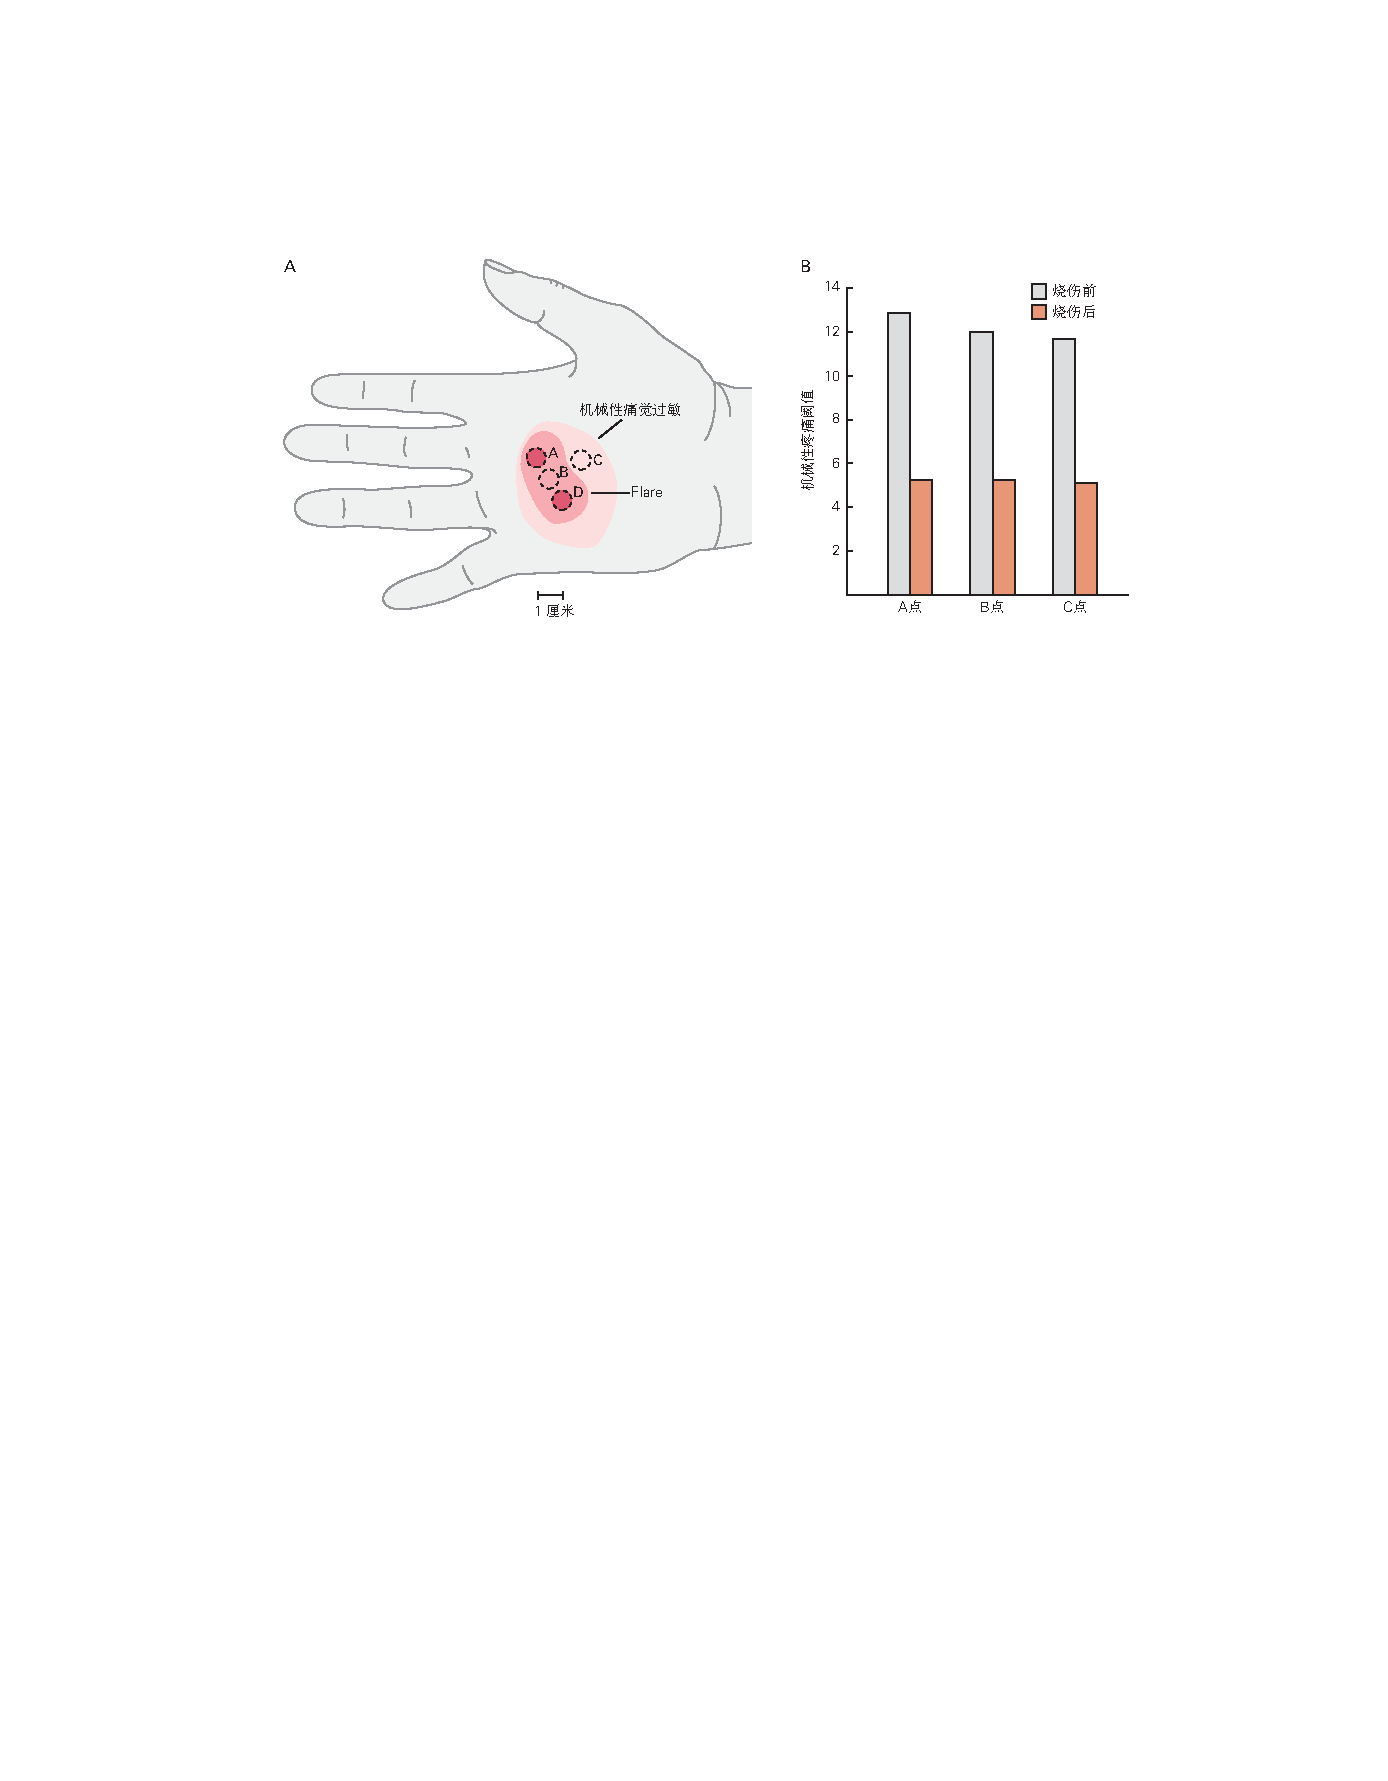
\includegraphics[width=0.7\linewidth]{chap20/fig_20_7}
	\caption{痛觉过敏是由伤害感受器的敏化引起的。 (经许可转载自 Raja、Campbell 和 Meyer,1984 年。版权所有 © 1984,牛津大学出版社。)
		A. 在 A 点和 D 点烧伤前后,记录了 A、B 和 C 点的机械疼痛阈值。 
		一名受试者的手上显示了由烧伤引起的发红(耀斑)和机械性痛觉过敏区域。 
		在所有受试者中,机械痛觉过敏的面积大于耀斑面积。 
		即使在耀斑消失后,机械性痛觉过敏仍然存在。 
		B. 烧伤前后的平均机械痛阈值。 
		烧伤后疼痛的机械阈值显着降低。}
	\label{fig:20_7}
\end{figure}

不受控制的伤害感受器激活与多种病理状况有关。
伤害感受器活动改变导致的两种常见疼痛状态是异常性疼痛和痛觉过敏。 
异常性疼痛患者对通常无害的刺激会感到疼痛:轻微抚摸晒伤的皮肤、类风湿性关节炎患者的关节运动,甚至是剧烈运动后早上起床的行为。 
然而,异常性疼痛患者不会持续感到疼痛; 
在没有外周刺激的情况下,就没有疼痛。 
相比之下,痛觉过敏患者——对伤害性刺激的过度反应——通常会在没有感觉刺激的情况下报告持续性疼痛。


持续性疼痛可分为两大类,伤害性疼痛和神经性疼痛。 
伤害性疼痛由皮肤或软组织中伤害感受器的激活引起,以响应组织损伤,并且通常伴随炎症发生。 
扭伤和拉伤会产生轻微形式的伤害性疼痛,而关节炎或侵入软组织的肿瘤会产生更严重的伤害性疼痛。 
通常,伤害性疼痛用非甾体类抗炎药(NSAIDS;见后面的讨论)治疗,或者在严重时用吗啡等阿片类药物治疗。


神经性疼痛由外周或中枢神经系统的神经直接损伤引起,通常伴有烧灼感或电击感。 
神经性疼痛包括复杂的局部疼痛综合征,即使是对肢体周围神经的非常轻微的损伤也会导致这种疼痛; 
带状疱疹后遗神经痛,许多患者在带状疱疹发作后经历的剧烈疼痛; 
或三叉神经痛,一种由三叉神经未知病理引起的面部剧烈、剧烈的疼痛。 
其他神经性疼痛包括肢体截肢后可能发生的幻肢痛(见图 \ref{fig:20_14})。 
在某些情况下,甚至可以在没有外周刺激的情况下发生自发的、持续的、通常是灼痛的疼痛,这种现象称为疼痛麻醉。 
在尝试通过消融三叉神经感觉神经元来治疗三叉神经痛后,可能会触发该综合征。 
神经性疼痛对非甾体抗炎药没有反应,通常对阿片类药物反应不佳。 
最后,中枢神经系统的损伤,例如多发性硬化、中风后或脊髓损伤后,也可导致中枢神经性疼痛状态。 
由于抑制性控制的丧失(如发生在癫痫中)是导致神经性疼痛的一个重要因素,因此毫不奇怪,神经性疼痛的一线治疗涉及抗惊厥药,尤其是加巴喷丁类药物。 
(提及 γ-氨基丁酸 [GABA] 是基于加巴喷丁与 GABA 的结构相似性。
然而,加巴喷丁实际上通过与电压门控 Ca2+ 通道的 α2δ-亚基结合发挥作用,最终减少神经递质释放。)

\begin{figure}[htbp]
	\centering
	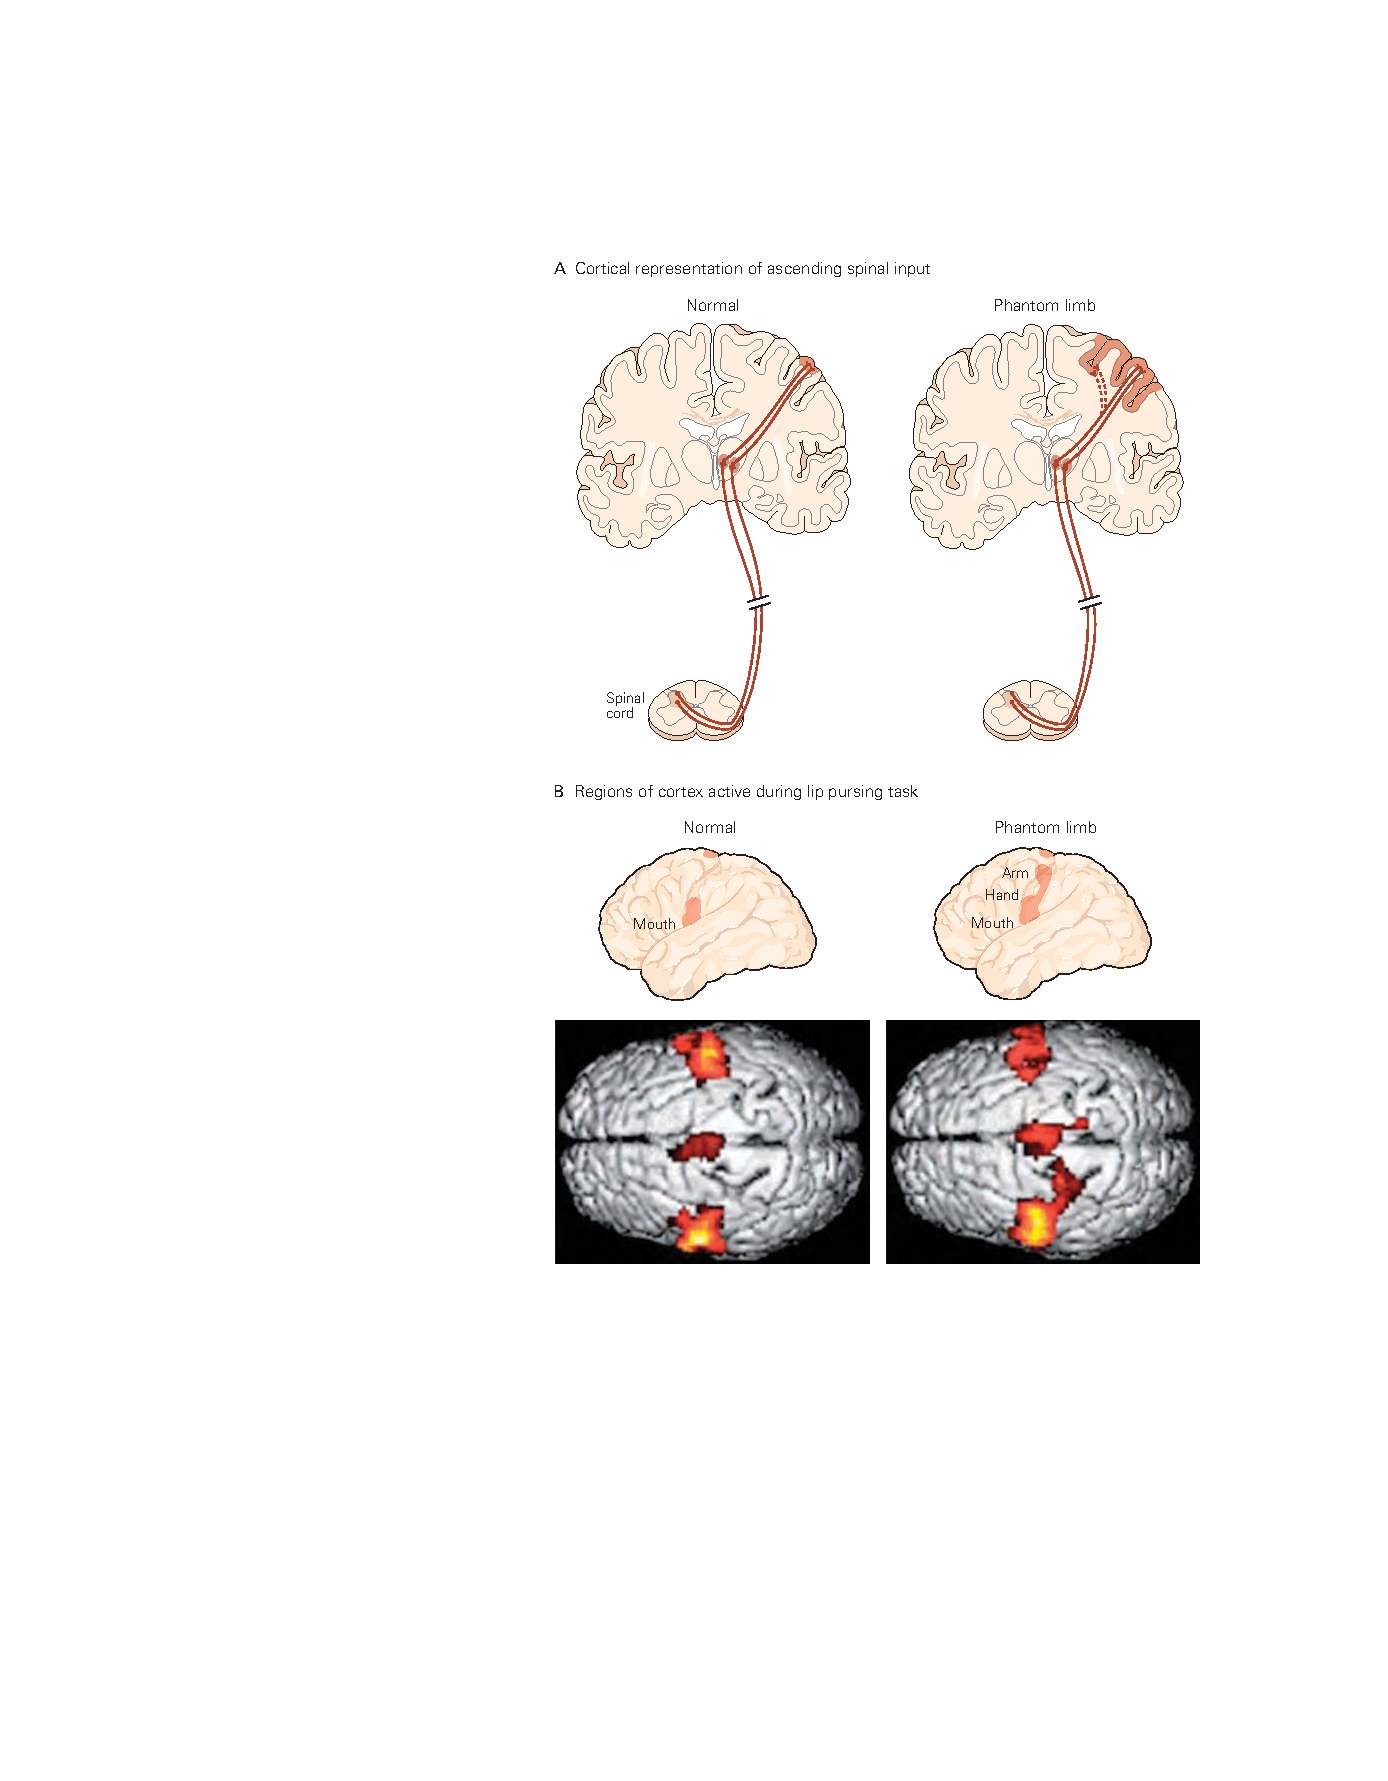
\includegraphics[width=0.7\linewidth]{chap20/fig_20_14}
	\caption{幻肢痛中神经激活的变化。 
		A. 在幻肢痛患者中,由上行脊髓感觉输入激活的大脑皮层区域扩大。 
		B. 幻肢痛患者和健康对照者在噘嘴任务期间的功能磁共振成像 (fMRI)。 
		在患有幻肢痛的截肢者中,嘴的皮质表征已经延伸到手和手臂的区域。 
		在没有疼痛的截肢者中,被激活的初级体感和运动皮层区域与健康对照组相似(图像未显示)。 (经许可改编自 Flor、Nokolajsen 和 Jensen,2006 年。版权所有 © 2006 Springer Nature。)}
	\label{fig:20_14}
\end{figure}


\section{来自伤害感受器的信号被传送到脊髓背角的神经元}
伤害性刺激的感觉来自伤害性感觉神经元的外周轴突分支中的信号,其细胞体位于背根神经节。
这些神经元的中央分支以高度有序的方式终止于脊髓。 
大多数终止于背角。
传递不同感觉方式的初级传入神经元终止于不同的薄层(图 \ref{fig:20_3} B),因此背角神经元的解剖组织、它们的接受特性和它们在感觉处理中的功能之间存在紧密联系。

\begin{figure}[htbp]
	\centering
	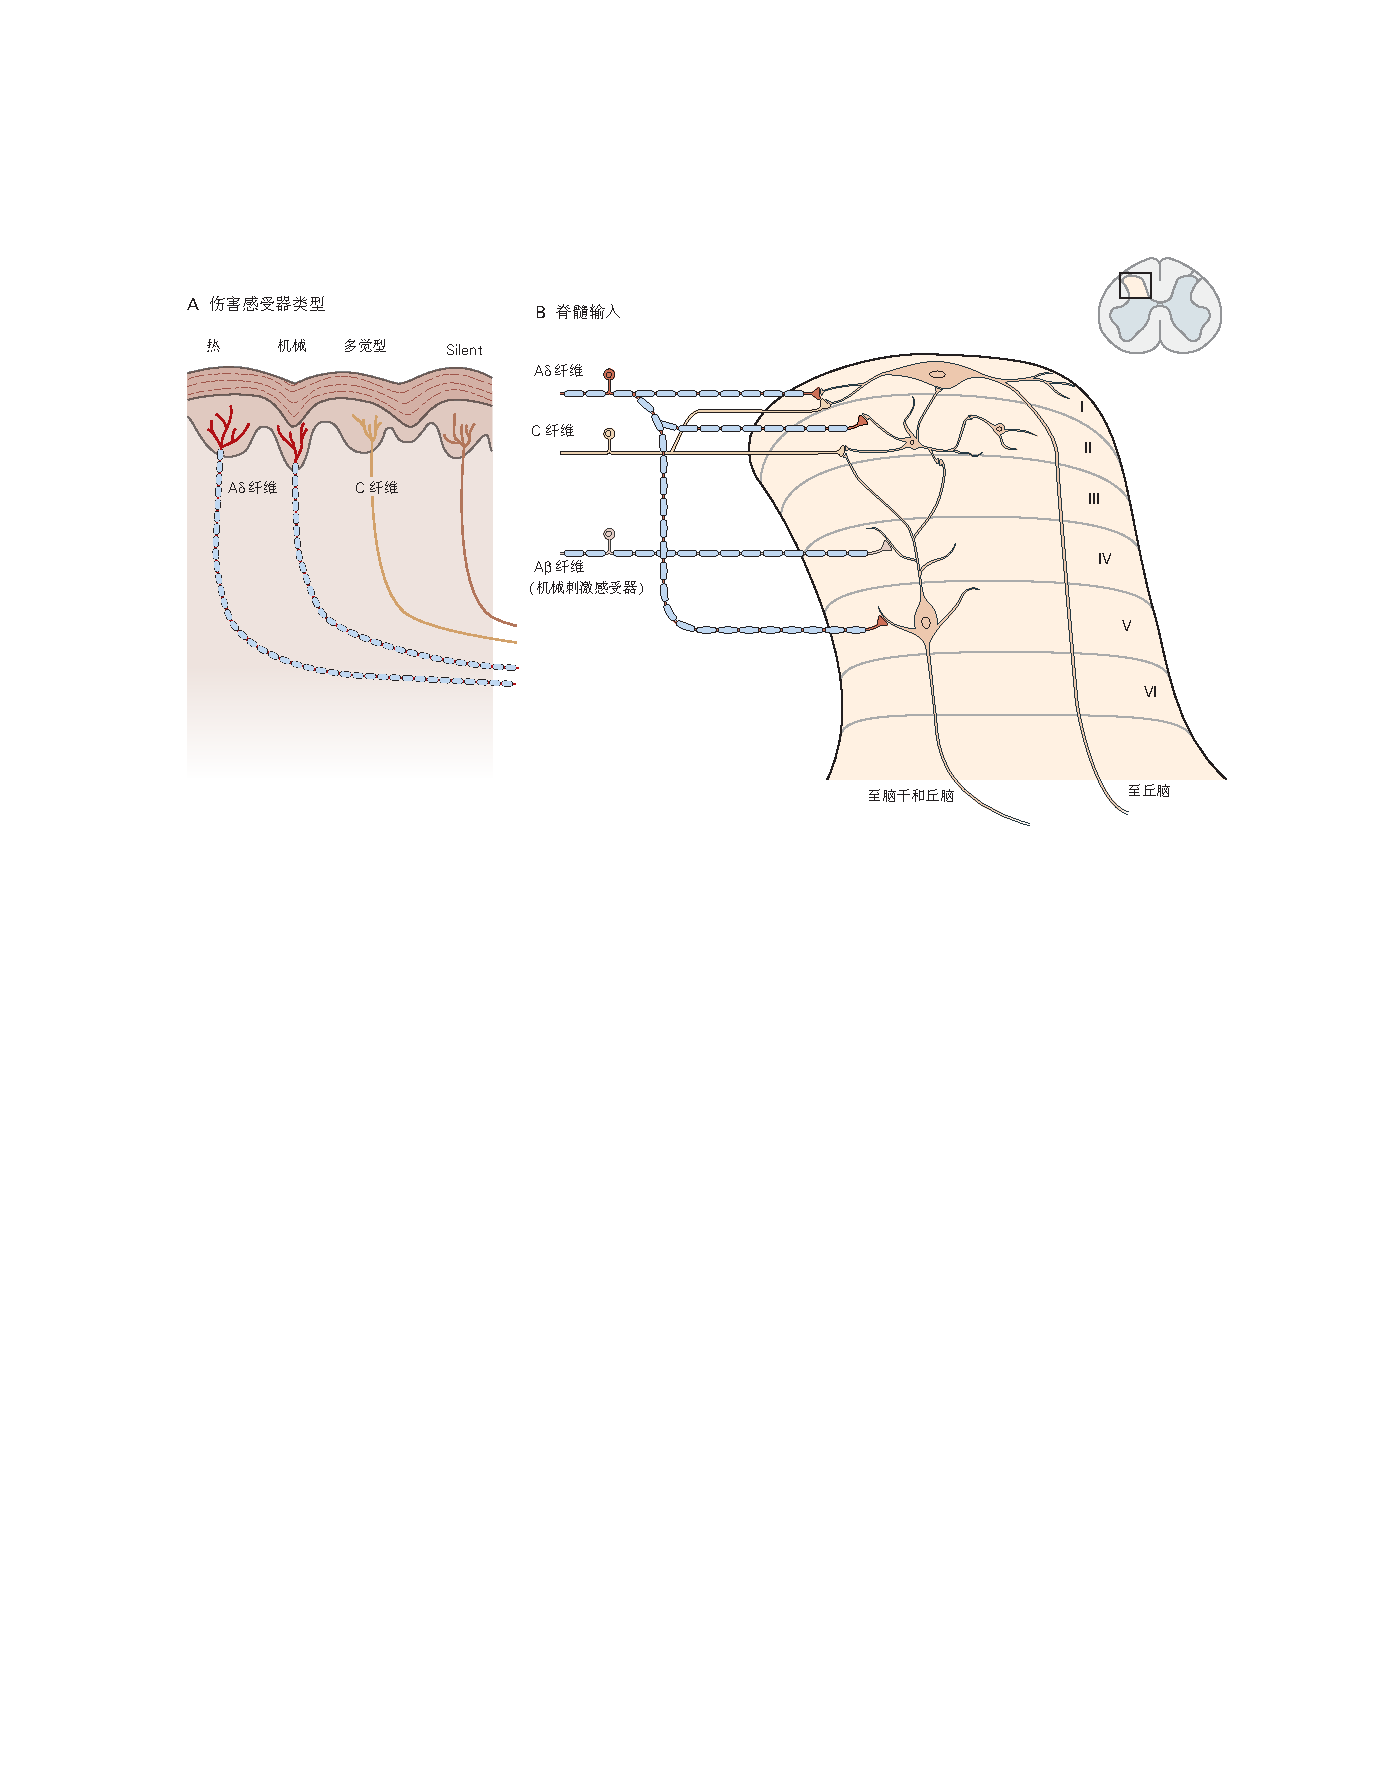
\includegraphics[width=0.7\linewidth]{chap20/fig_20_3}
	\caption{伤害感受纤维终止于脊髓背角的不同层。 
		A. 外周伤害感受器和无声伤害感受器主要分为三类,它们由炎症和各种化学物质激活。 
		B. 背角 I 层中的神经元通过层 II 中的中间神经元接收来自有髓 (Ac) 伤害感受纤维的直接输入以及来自无髓 (C) 伤害感受纤维的直接和间接输入。 
		Lamina V 神经元接收来自大直径有髓鞘 Aβ 机械感受纤维的低阈值输入以及来自伤害性 Aδ 和 C 纤维的输入。 
		Lamina V 神经元将树突发送到 lamina IV,在那里它们与 Aβ 初级传入神经的末端接触。 
		II 层中间神经元的轴突末端可以与由 V 层细胞产生的 III 层中的树突接触。
		Aα 初级传入神经接触腹侧脊髓中的运动神经元和中间神经元(未显示)。 (经许可改编自 Fields 1987。)}
	\label{fig:20_3}
\end{figure}


背角最表层的许多神经元,称为 I 层或边缘层,对 Aδ 和 C 纤维传递的有害刺激有反应。 
因为它们选择性地对伤害性刺激做出反应,所以它们被称为伤害感受特异性神经元。 
这组神经元投射到中脑和丘脑。 
第二类 I 层神经元接收来自 C 纤维的输入,这些 C 纤维被冷刺激选择性激活。 
其他类别的 I 层神经元以分级方式对无害和有害的机械刺激作出反应,因此被称为宽动态范围神经元。


Lamina II,即明胶质,是一个密集层,包含许多不同类别的局部中间神经元,一些是兴奋性的,另一些是抑制性的。 
这些中间神经元中的一些选择性地响应引起疼痛的输入,而另一些则选择性地被引起瘙痒的刺激激活。 
Laminae III 和 IV 含有局部中间神经元和脊髓上投射神经元的混合物。 
许多这些神经元接收来自 Aβ 传入纤维的输入,这些传入纤维对无害的皮肤刺激有反应,例如毛发的偏转和光压。 
Lamina V 包含对各种有害刺激做出反应并投射到脑干和丘脑的神经元。 
这些神经元接收来自 Aβ 和 Aδ 纤维的直接输入,并且由于它们的树突延伸到第 II 层,也由 C 纤维伤害感受器支配(图 \ref{fig:20_3} B)。


椎板 V 中的神经元也接收来自内脏组织中伤害感受器的输入。 
躯体和内脏伤害性输入对单个椎板 V 神经元的聚合为称为“牵涉痛”的现象提供了一种解释,在这种情况下,内脏组织受伤引起的疼痛被认为起源于身体表面的某个区域。 
例如,心肌梗塞患者经常报告左臂和胸部疼痛(图 \ref{fig:20_4})。 
这种现象的发生是因为单个 V 层神经元从两个区域接收感觉输入,因此来自该神经元的信号不会通知更高的大脑中枢有关输入源的信息。 
因此,大脑经常错误地将疼痛归因于皮肤,这可能是因为皮肤输入占主导地位。 
对牵涉痛实例的另一种解剖学解释是,伤害性感觉神经元的轴突在周围分支,支配皮肤和内脏目标。


\begin{figure}[htbp]
	\centering
	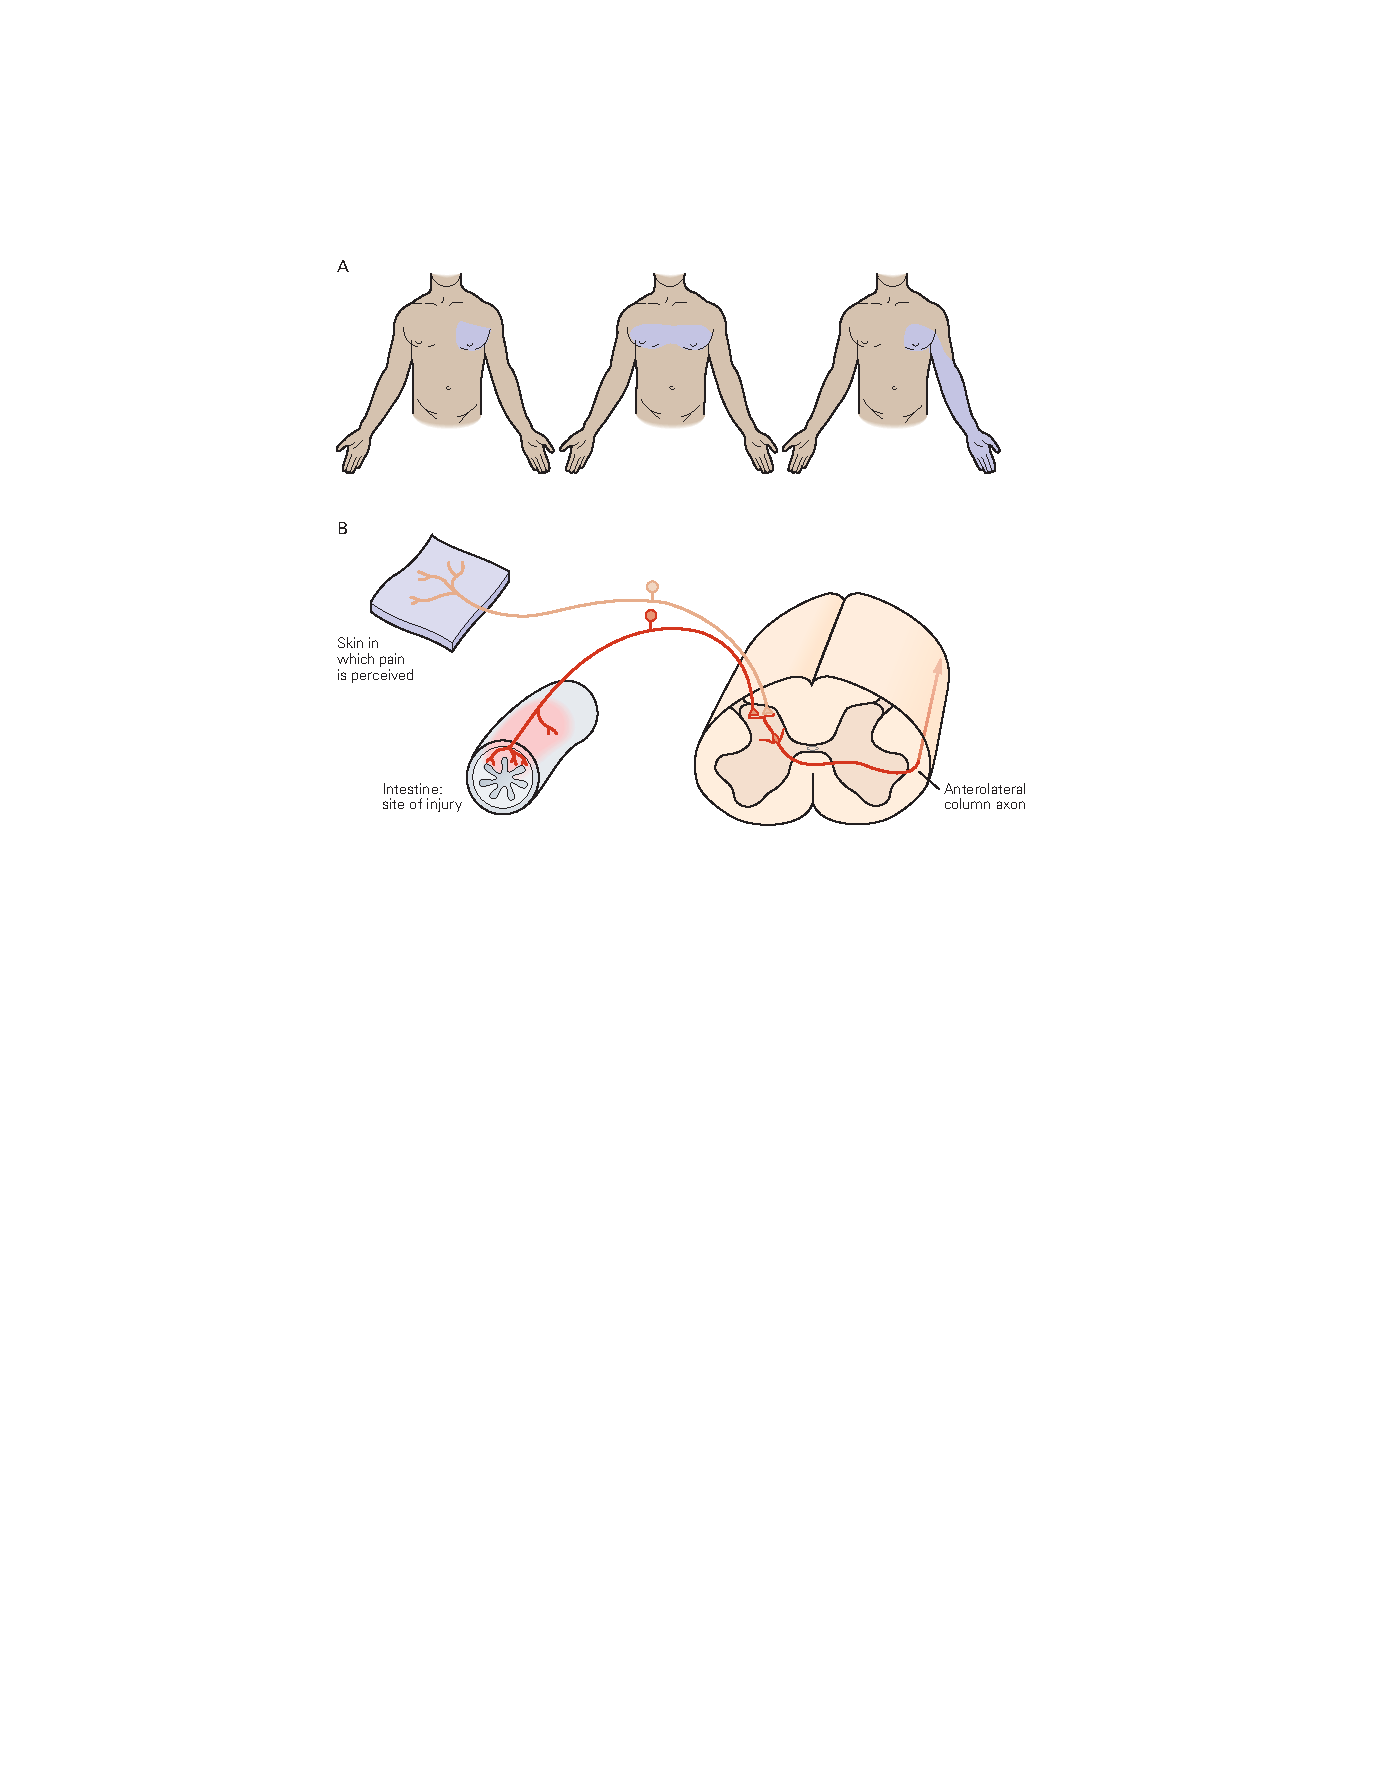
\includegraphics[width=0.7\linewidth]{chap20/fig_20_4}
	\caption{来自内脏伤害感受器的信号可以在身体其他部位被感知为“牵涉痛”。 
		A. 心肌梗塞和心绞痛可表现为胸部和左臂的深部牵涉痛。 
		从牵涉痛的部位不能很容易地预测疼痛的来源。 
		B. 内脏和躯体传入纤维的会聚可能是牵涉痛的原因。 
		来自内脏的伤害性传入纤维和来自皮肤特定区域的纤维会聚在背角的相同投射神经元上。 
		大脑无法知道有害刺激的实际位置,并且错误地将来自内脏器官的信号与皮肤区域相关联。 (经许可改编自 Fields 1987。)}
	\label{fig:20_4}
\end{figure}

第六层神经元接收来自支配肌肉和关节的大直径初级传入纤维的输入。 
这些神经元由无害的关节运动激活,不参与伤害性信息的传递。 
VII 和 VIII 层(脊髓的中间和腹侧区域)中的许多神经元确实对伤害性刺激有反应。 
这些神经元通常具有复杂的响应特性,因为从伤害感受器到这些神经元的输入是通过许多中间突触传递的。 
椎板 VII 中的神经元通常对身体任一侧的刺激作出反应,而大多数背角神经元接收单侧输入。 
因此,人们认为第 VII 层神经元的激活有助于许多疼痛状况的弥散性。


激活脊髓背角神经元的伤害性感觉神经元释放两大类神经递质。 
谷氨酸是所有初级感觉神经元的主要神经递质,无论感觉方式如何。 
神经肽作为协同递质被许多带有无髓鞘轴突的伤害感受器释放。 
这些肽包括 P 物质、降钙素基因相关肽 (CGRP)、生长抑素和甘丙肽(图 \ref{fig:20_5})。 
谷氨酸储存在小的、电子透明的囊泡中,而肽则被隔离在伤害性感觉神经元中央末端的大的、致密的核心囊泡中(图 \ref{fig:20_6})。 
不同的存储位置允许这两类神经递质在不同的生理条件下有选择地释放。

\begin{figure}[htbp]
	\centering
	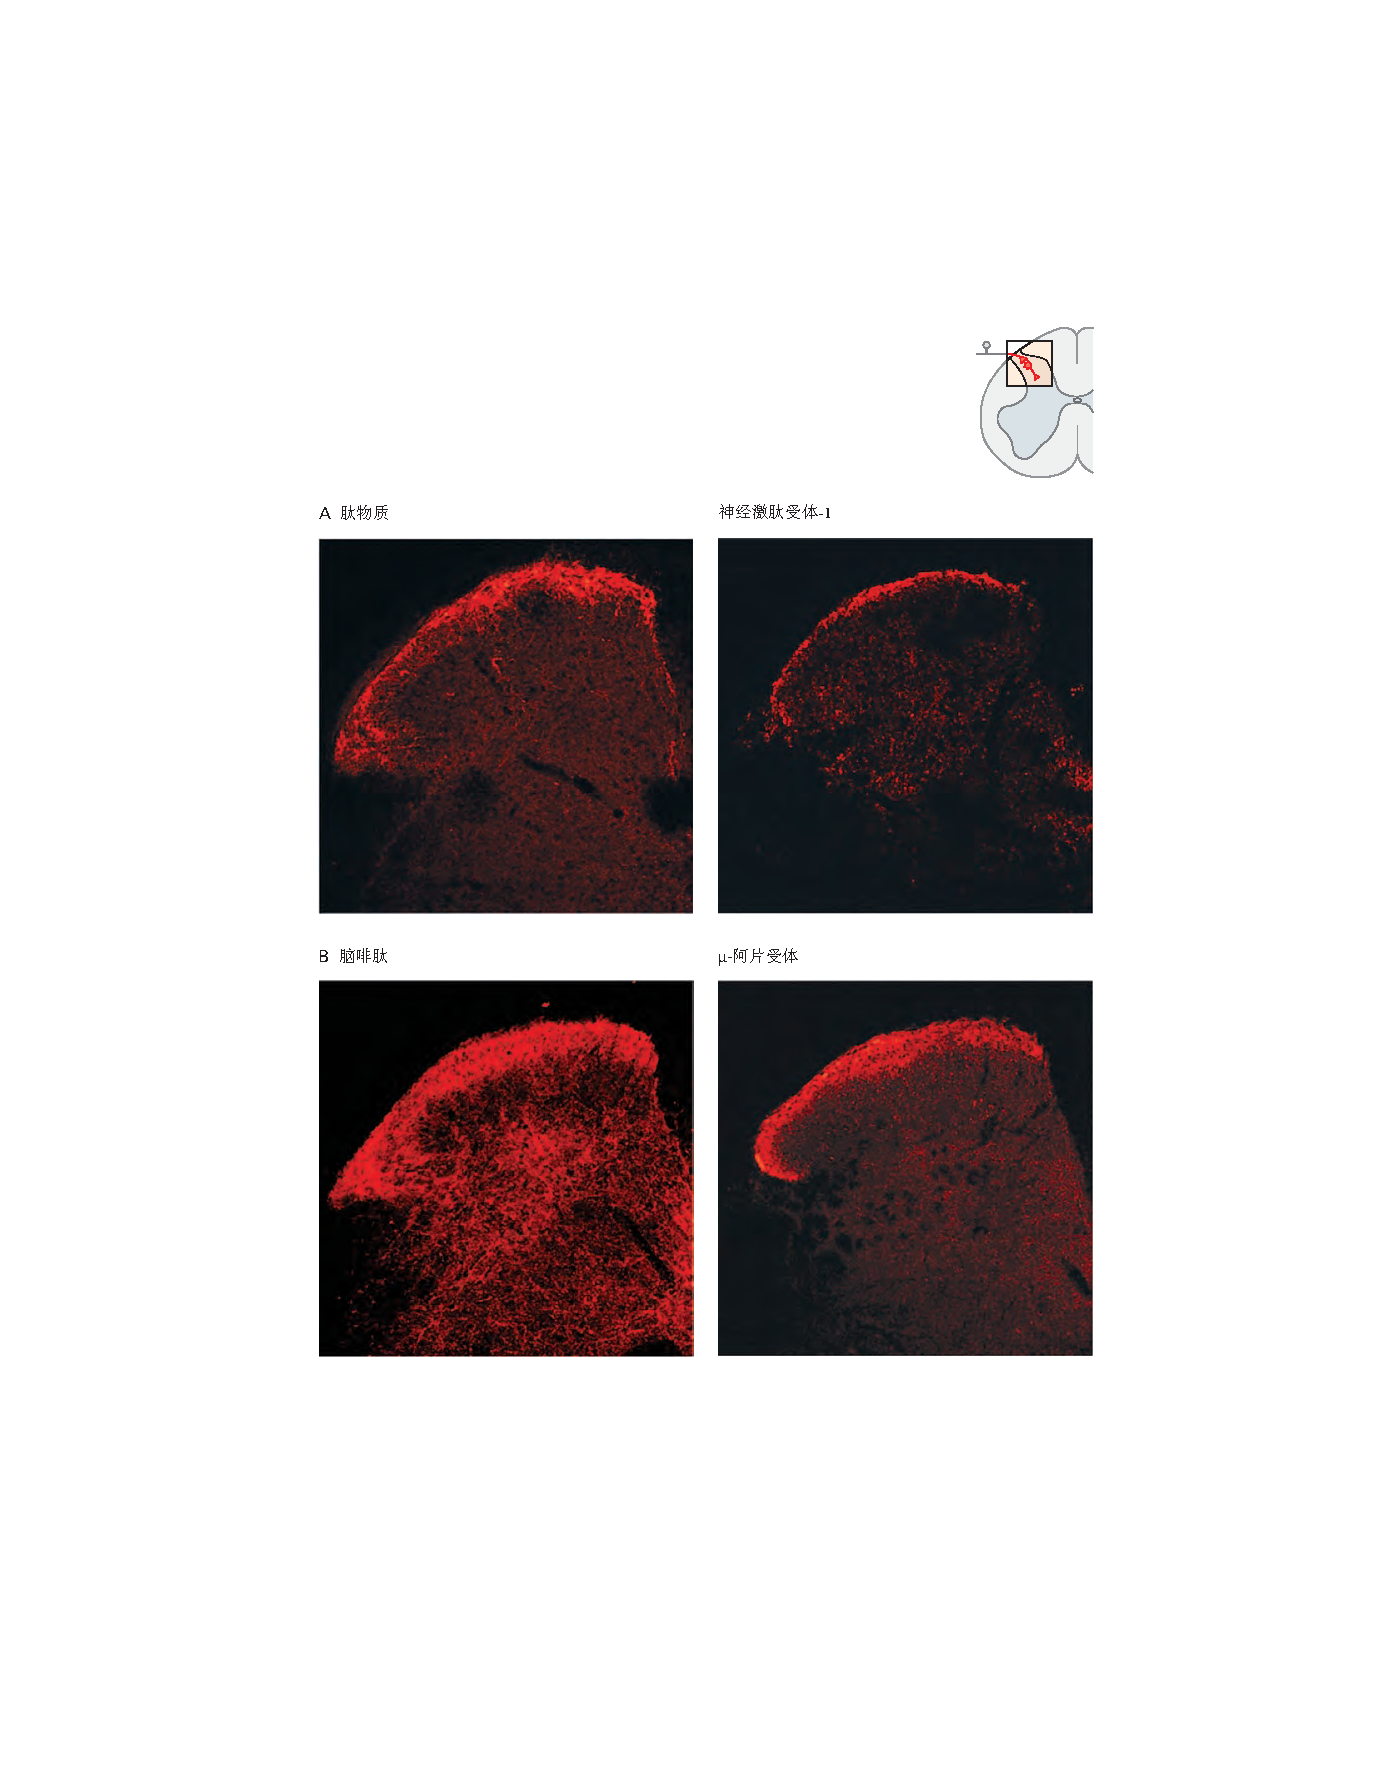
\includegraphics[width=0.7\linewidth]{chap20/fig_20_5}
	\caption{大鼠脊髓浅背角的神经肽及其受体。 (图像经 A. Basbaum 许可转载。) 
		A. 无髓鞘初级感觉神经元的末端是浅表背角中 P 物质的主要来源。 
		P 物质激活神经激肽 1 (NK1) 受体,该受体由浅表背角中的神经元表达,其中大部分是投射神经元。 
		B. 脑啡肽位于中间神经元中,发现与含有 P 物质的末梢位于同一区域。 
		感觉神经元的末梢。}
	\label{fig:20_5}
\end{figure}


\begin{figure}[htbp]
	\centering
	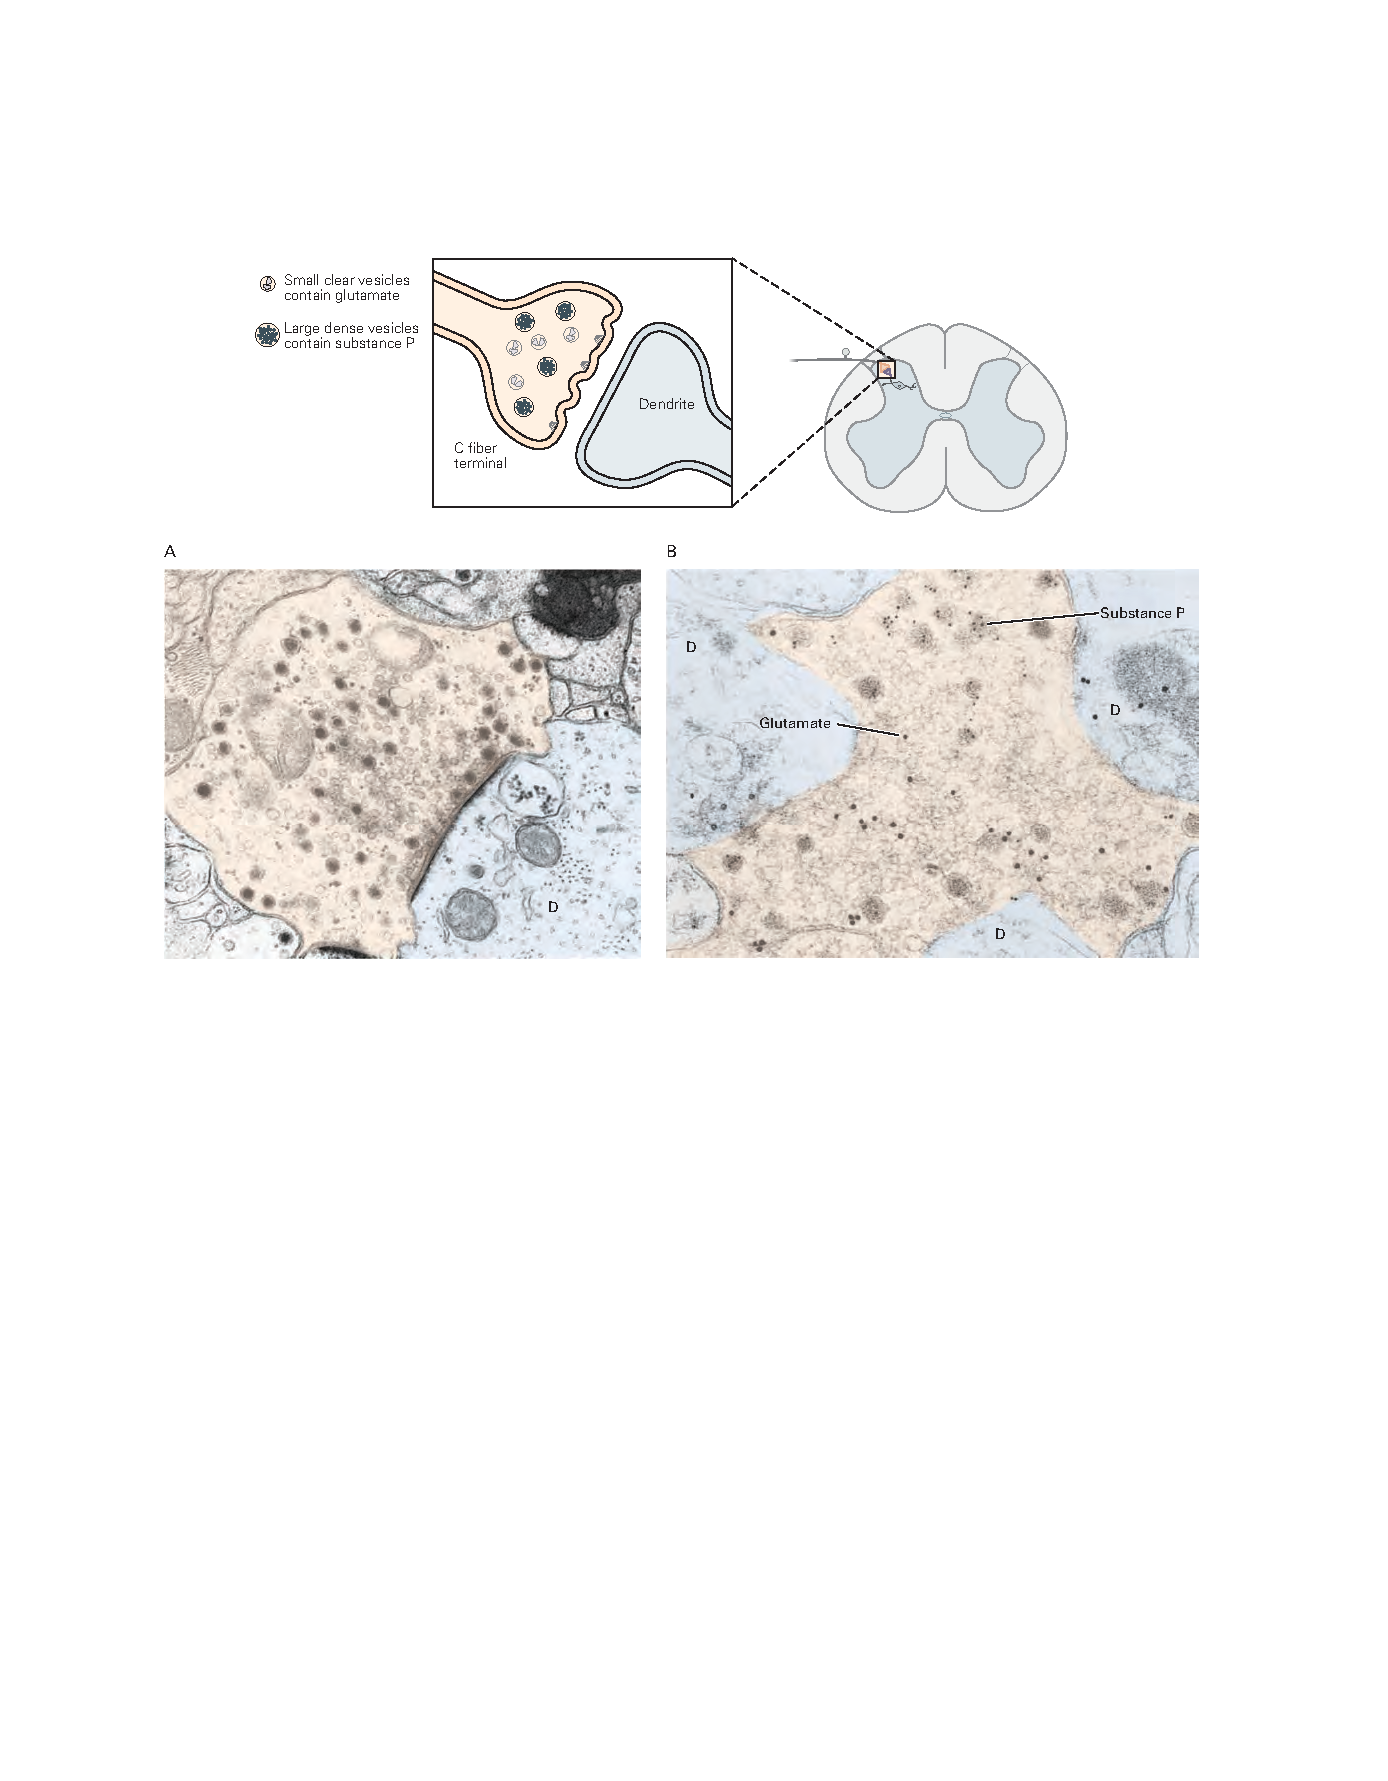
\includegraphics[width=0.7\linewidth]{chap20/fig_20_6}
	\caption{背侧脊髓初级伤害性神经元突触末端的递质存储。 
		A. 背角神经元树突 (D) 上的 C 纤维末端有两类包含不同递质的突触小泡。 
		小的电子透明囊泡含有谷氨酸,而大的致密核囊泡储存神经肽。 (图像经许可转载自 H. J. Ralston III。)
		B. 谷氨酸和肽物质 P(分别以大金粒和小金粒标记)散布在背角 II 层感觉神经元末梢的轴浆中。 
		致密核心囊泡还储存降钙素基因相关肽 (CGRP)。 (经许可转载自 De Biasi 和 Rustioni 1990。)}
	\label{fig:20_6}
\end{figure}


在伤害性感觉神经元释放的神经肽递质中,对神经激肽家族成员 P 物质的作用进行了最详细的研究。 
P 物质在组织损伤或周围神经强烈刺激后从伤害性传入神经的中央末端释放。 
它与背角神经元上的神经激肽受体的相互作用引起缓慢的兴奋性突触后电位,从而延长谷氨酸引起的去极化。 
尽管谷氨酸和神经肽对背角神经元的生理作用不同,但这些递质协同作用以调节背角神经元的放电特性。


神经肽与其在背角神经元上的受体相互作用的细节为慢性疼痛调节提出了策略。 
将与神经毒素偶联的 P 物质输注到实验动物的背角会导致表达神经激肽受体的神经元的选择性破坏。 
以这种方式治疗的动物无法产生通常与外周损伤相关的中枢敏化。 
这种神经元消融方法比部分脊髓横断(前外侧脊髓切开术)等传统外科手术更具选择性,并且被认为是治疗患有其他顽固性慢性疼痛的患者的方法。



\section{痛觉过敏既有外周起源也有中枢起源}
到目前为止,我们已经考虑了正常生理状态下有害信号的传递。 
但是当外周组织受损时,感觉信号的正常过程会发生显着变化,从而导致疼痛敏感性或痛觉过敏增加。 
这种情况可以通过反复暴露于伤害性刺激而使外周伤害感受器敏感而引发(图 \ref{fig:20_7})。


致敏作用是由聚集在组织损伤部位的受损细胞释放的复杂化学物质混合物引发的。 
这种混合物含有肽和蛋白质,如缓激肽、P 物质和神经生长因子,以及分子,如 ATP、组胺、血清素、前列腺素、白三烯和乙酰胆碱。 
这些化学介质中有许多是从不同的细胞类型中释放出来的,但它们共同作用会降低伤害感受器激活的阈值。


这些化学物质从何而来,它们究竟有什么作用? 
组胺在组织损伤后从肥大细胞中释放出来并激活多模式伤害感受器。 
脂质 anandamide 是一种内源性大麻素激动剂,在炎症条件下释放,激活 TRPV1 通道,并可能引发与炎症相关的疼痛。 
ATP、乙酰胆碱和血清素从受损的内皮细胞和血小板中释放出来; 它们通过触发外周细胞释放前列腺素和缓激肽等化学物质,间接使伤害感受器敏感。


缓激肽是最活跃的止痛剂之一。 
它的效力部分源于这样一个事实,即它直接激活 Aδ 和 C 伤害感受器并增加附近细胞前列腺素的合成和释放。 
前列腺素是花生四烯酸的代谢产物,它是通过环氧合酶 (COX) 酶的活性裂解花生四烯酸而产生的(第 14 章)。 
COX-2 酶优先在外周炎症条件下被诱导,有助于增强疼痛敏感性。 
前列腺素合成的酶促途径是常用镇痛药物的靶点。 
阿司匹林和其他非甾体抗炎镇痛药(如布洛芬和萘普生)可有效控制疼痛,因为它们可阻断 COX 酶的活性,减少前列腺素的合成。


外周伤害感受器的活动也会产生炎症的所有主要体征,包括发热(发热)、发红(红肿)和肿胀(肿瘤)。 
热和发红是由外周血管扩张引起的,而肿胀是由血浆外渗引起的,在这个过程中,蛋白质、细胞和液体能够穿透毛细血管后微静脉。 
从 C 纤维的外周末端释放神经肽物质 P 和 CGRP 分别引起血浆外渗和血管舒张。 
因为这种形式的炎症取决于神经活动,所以它被称为神经源性炎症(图 \ref{fig:20_8})。 
重要的是,由于严重的外周血管扩张是许多偏头痛的关键触发因素,因此通过清除 CGRP 来抵消血管扩张的 CGRP 抗体的开发为新的偏头痛治疗提供了巨大的希望。

\begin{figure}[htbp]
	\centering
	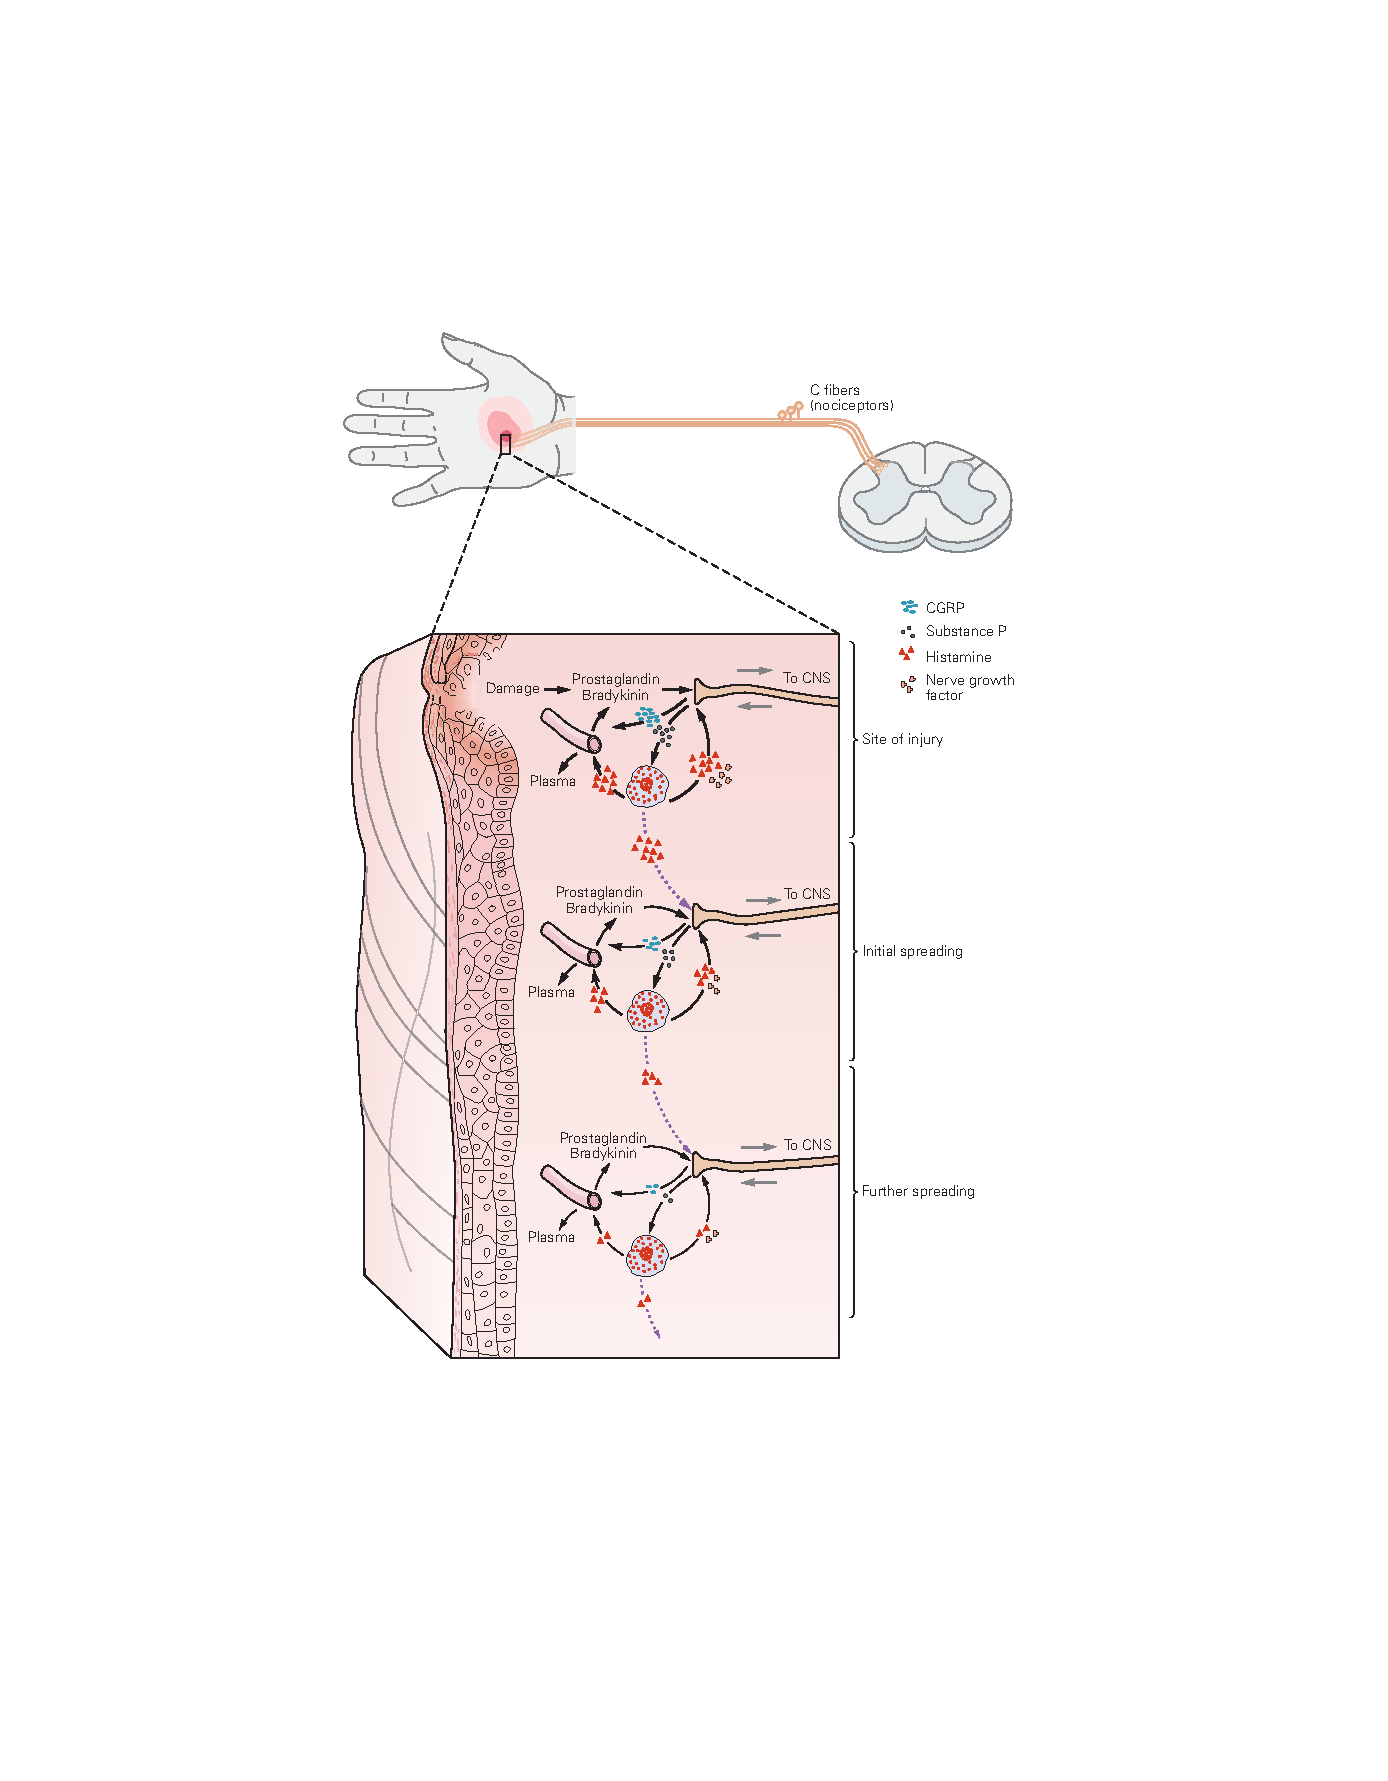
\includegraphics[width=0.7\linewidth]{chap20/fig_20_8}
	\caption{神经源性炎症。 
		损伤或组织损伤会释放缓激肽和前列腺素,它们会激活伤害感受器或使伤害感受器敏感。 
		伤害感受器的激活导致 P 物质和降钙素基因相关肽 (CGRP) 的释放。 
		P 物质作用于感觉末梢附近的肥大细胞(浅蓝色),引起脱颗粒和组胺释放,直接刺激伤害感受器。 
		P物质还产生血浆外渗和水肿,CGRP产生外周血管扩张(导致皮肤发红); 由此产生的炎症导致缓激肽的额外释放。 
		这些机制也发生在健康组织中,它们会导致继发性或扩散性痛觉过敏。 (缩写:CNS,中枢神经系统。)}
	\label{fig:20_8}
\end{figure}

感觉神经元末梢 P 物质和 CGRP 的释放也是轴突反射的原因,轴突反射是一种以皮肤损伤附近的血管舒张为特征的生理过程。 
P 物质的药理学拮抗剂能够阻断人类的神经源性炎症和血管舒张; 这一发现说明了如何将伤害性机制的知识应用于改善疼痛的临床治疗。


除了这些小分子和肽外,神经营养素也是疼痛的致病因子。 
神经生长因子 (NGF) 和脑源性神经营养因子 (BDNF) 在炎症性疼痛状态下特别活跃。 
BDNF 的合成在许多发炎的外周组织中上调(图 \ref{fig:20_9} )。 
NGF 中和分子在持续性疼痛的动物模型中是有效的镇痛剂。 
事实上,NGF 功能和信号传导的抑制与 COX 抑制剂和阿片类药物一样有效地阻断痛觉。 
已经报道了几项使用 NGF 抗体治疗膝骨关节炎的有前途的临床试验,再次证明了基础科学向临床的转化。


\begin{figure}[htbp]
	\centering
	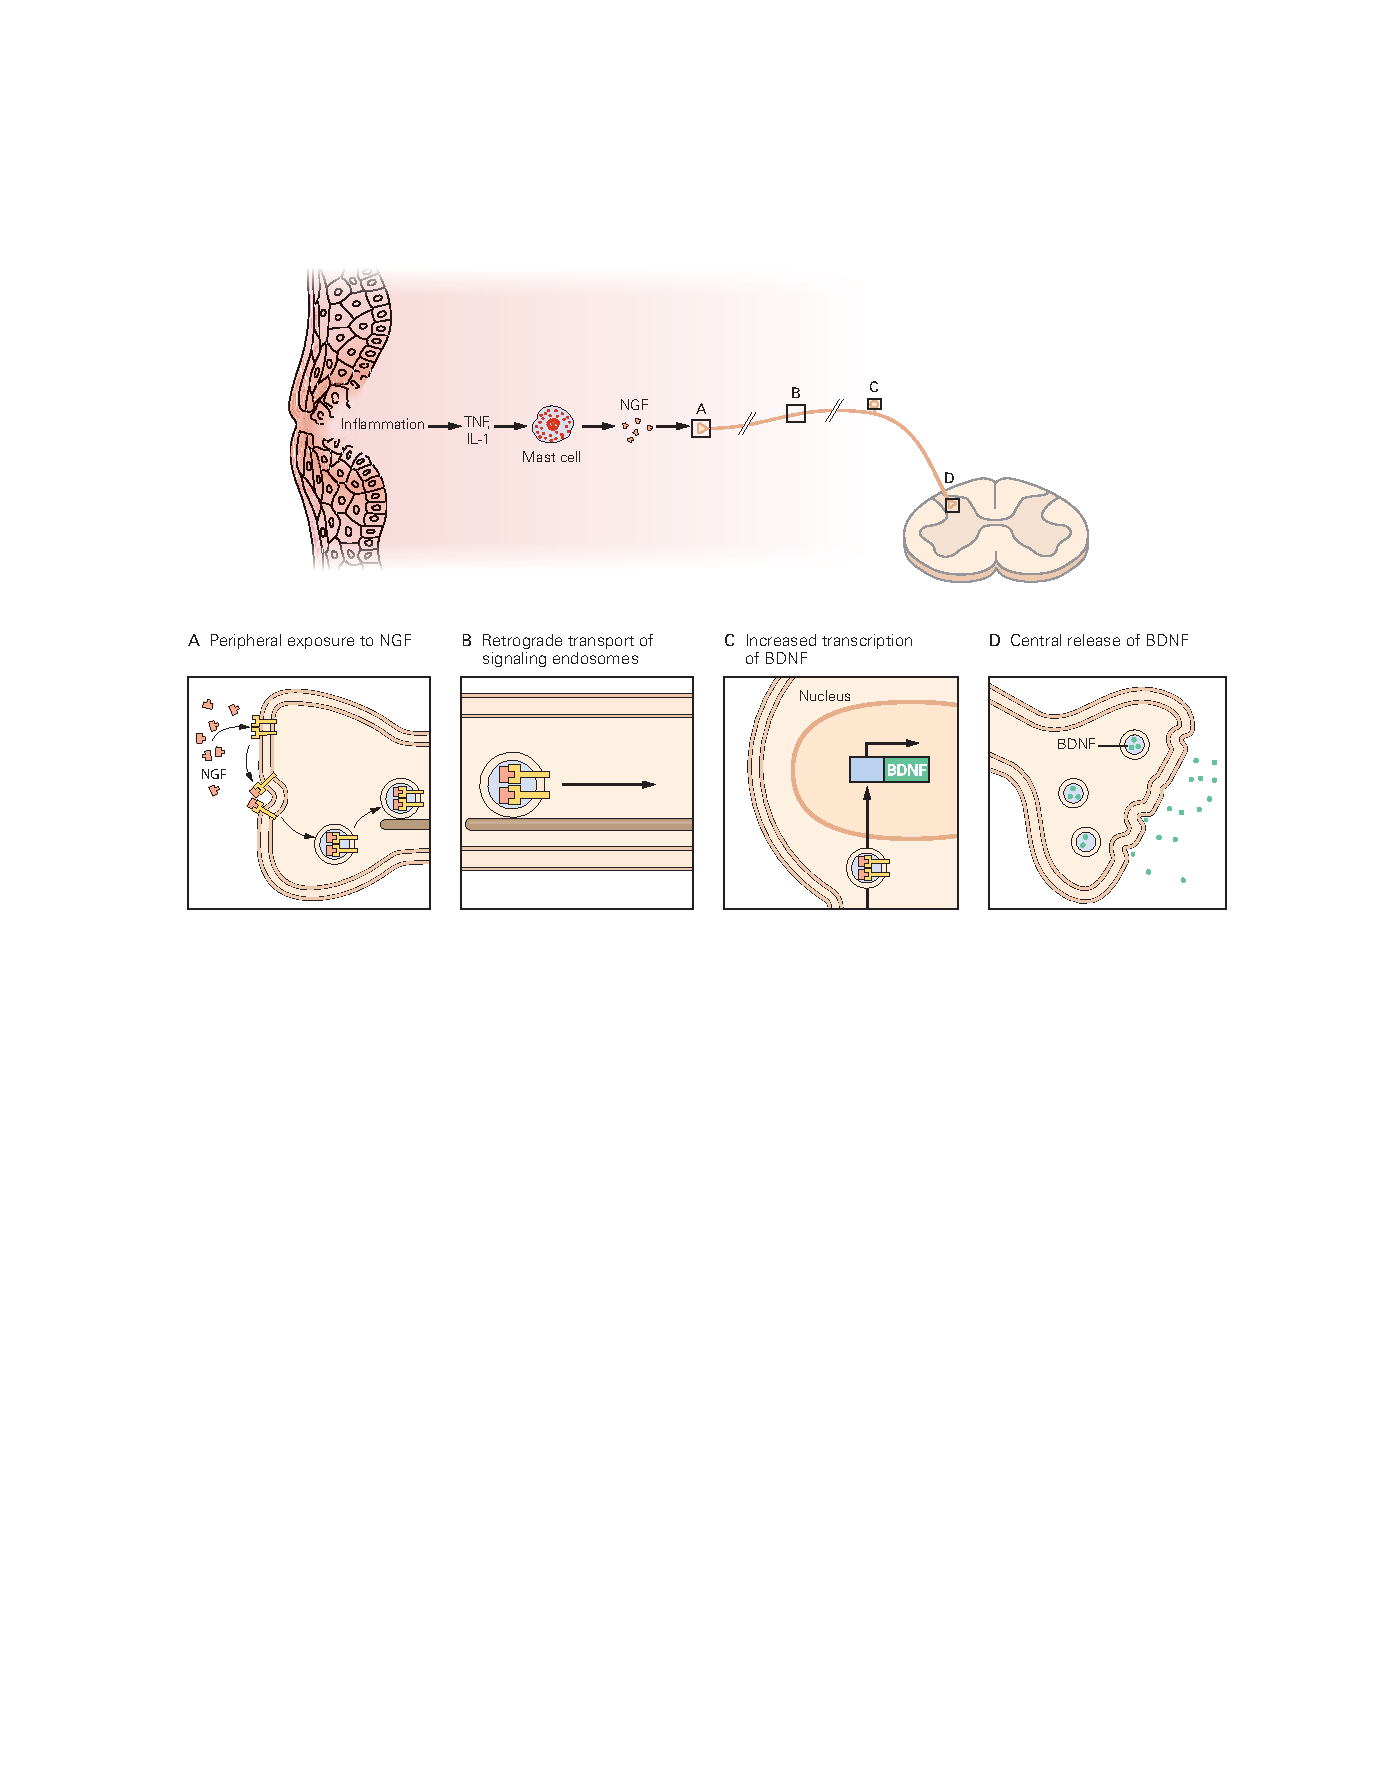
\includegraphics[width=0.7\linewidth]{chap20/fig_20_9}
	\caption{神经营养素是疼痛介质。 
		白细胞介素 1 (IL-1) 和肿瘤坏死因子 (TNF) 等炎性细胞因子的局部产生促进了外周几种细胞类型的神经生长因子 (NGF) 的合成和释放。 
		神经生长因子与初级伤害感受器末梢 (A) 上的 TrkA 受体结合,引发离子通道表达的上调,从而增加伤害感受器的兴奋性。 
		信号内体向细胞体的逆行转运 (B) 导致脑源性神经营养因子 (BDNF) (C) 的表达增强,并且它从脊髓中的感觉末梢释放 (D) 进一步增加了背角神经元的兴奋性。}
	\label{fig:20_9}
\end{figure}

是什么导致了背角神经元对伤害感受器信号的敏感性增强? 
在持续性损伤的情况下,C 纤维反复放电,背角神经元的反应逐渐增加(图 \ref{fig:20_10} A)。 
背角神经元兴奋性的逐渐增强被称为“饱和”,被认为涉及 N-甲基-d-天冬氨酸 (NMDA) 型谷氨酸受体(图 \ref{fig:20_10} B)。

\begin{figure}[htbp]
	\centering
	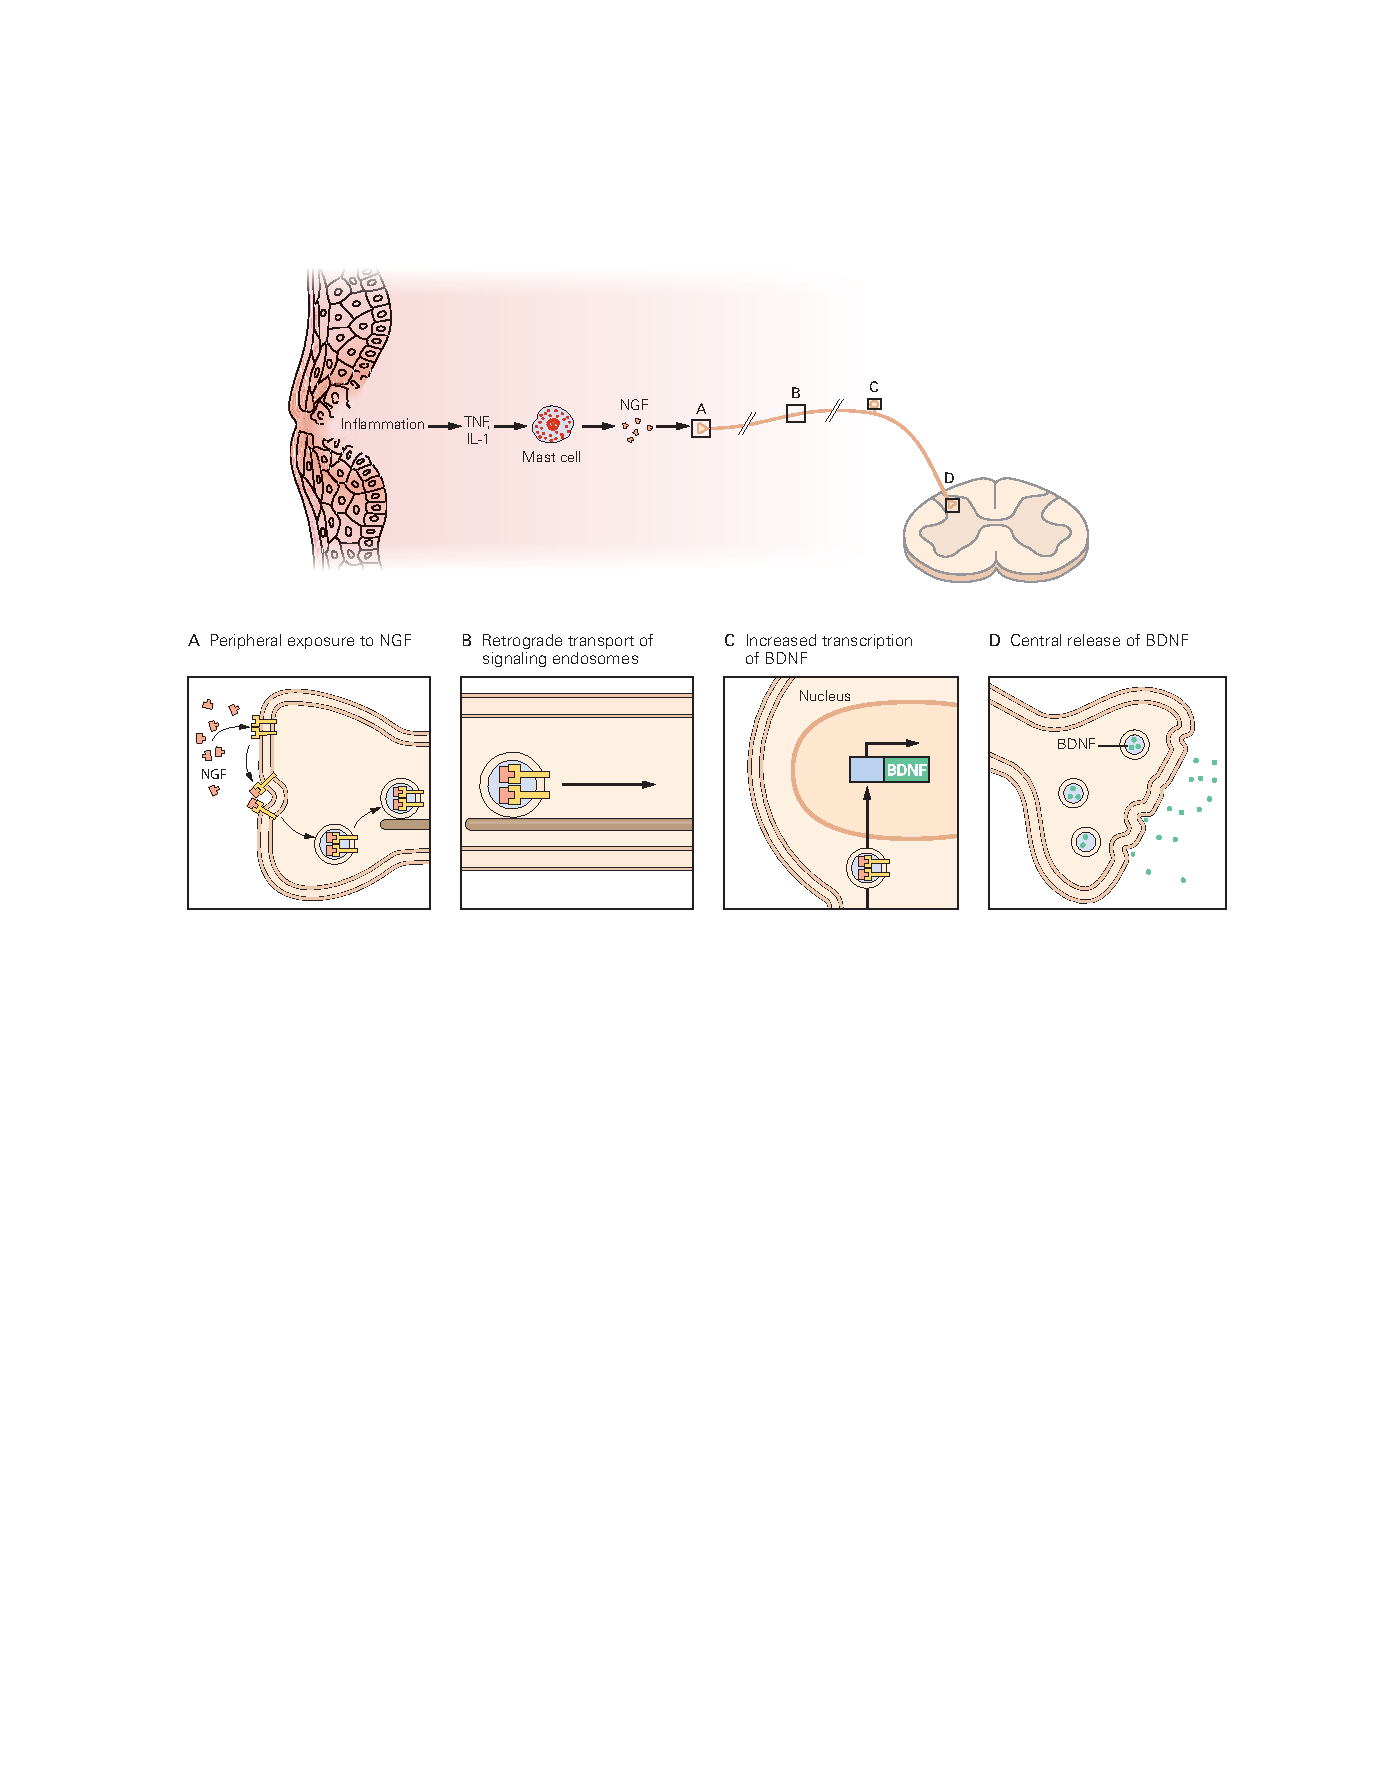
\includegraphics[width=0.7\linewidth]{chap20/fig_20_9}
	\caption{增强背角神经元兴奋性的机制。 
		A. 大鼠背角神经元对以 1 Hz 频率经皮传递的电刺激的典型反应。 随着重复刺激,C 纤维诱发的长潜伏期成分逐渐增加,而 A 纤维诱发的短潜伏期成分保持不变。 
		B. 背角神经元接收来自 Aδ 和 C 纤维伤害感受器的单突触和多突触输入。 
		突触前末端残留 Ca2+ 的升高导致谷氨酸和 P 物质(和 CGRP,未显示)的释放增加。
		左图:Aδ 纤维激活突触后 AMPA 受体导致快速瞬时膜去极化,从而减轻 NMDA 受体的 Mg2+ 阻滞。 
		右图:C 纤维激活突触后 NMDA 受体和神经激肽 1 (NK1) 受体会产生持久的累积去极化。 
		由于 Ca2+ 通过 NMDA 受体通道和电压敏感 Ca2+ 通道进入,因此背角神经元中的细胞溶质 Ca2+ 浓度增加。 
		第二信使系统的 Ca2+ 升高和 NK1 受体的激活增强了 NMDA 受体的性能。 
		NK1 受体的激活、累积去极化、细胞溶质 Ca2+ 升高和其他因素调节负责动作电位的电压门控离子通道的行为,导致兴奋性增强,所有这些都有助于中枢敏化过程。 (缩写:AMPA,α-amino-3-hydroxy-5-methylisoxazole-4-propionate;NMDA,N-methyl-d-aspartate)}
	\label{fig:20_10}
\end{figure}

因此,反复暴露于有害刺激会导致背角神经元的反应发生长期变化,其机制类似于大脑中许多回路中突触反应长期增强的机制。 
本质上,背角神经元兴奋性的这些长期变化构成了 C 纤维输入状态的“记忆”。 
这种现象被称为中枢敏化,以区别于背角神经元外周末端的敏化,后者是一种涉及激活前列腺素合成酶途径的过程。


背角神经元的致敏还涉及第二信使通路的募集和与中枢神经系统其他区域的记忆存储有关的蛋白激酶的激活。 
这种酶促级联的结果之一是编码转录因子(如 c-fos)的早期基因的表达,这些基因被认为可以激活效应蛋白,使背角神经元对感觉输入敏感。 
最重要的是,背角“疼痛”传输回路的中枢敏化是可以降低疼痛阈值(异常性疼痛)并导致自发性疼痛(即在没有外周刺激的情况下持续疼痛)的过程。


中枢敏化也是由于神经损伤引起的神经性疼痛的主要原因。 
同样,NMDA 受体介导的背角回路的兴奋性增加。 
背角也失去了抑制控制。 
在正常情况下,背角中的 GABA 能抑制性中间神经元不仅具有强直活性,而且还被大直径、非伤害性 Aβ 纤维的活性激活(图 \ref{fig:20_11} A)。 
外周神经损伤会降低 GABA 能控制,从而加剧这些伤害性通路的过度活跃(图 \ref{fig:20_11} B)。 
最近的研究还表明神经损伤诱导的小胶质细胞激活以及随之而来的中枢致敏过程中 GABA 能抑制的减少(图 \ref{fig:20_11} C 和 20-12)。 
这些变化共同导致机械异常性疼痛(即通常无害的机械刺激引起的疼痛)。 
由于 Aβ 有髓鞘传入神经对背角伤害性通路回路的不当参与,机械性异常性疼痛也会发生。 
事实上,可能会发生疼痛扩散(继发性痛觉过敏),因为受伤区域外未受伤的 Aβ 传入神经会不适当地激活已经发生中枢敏化的背角回路。


\begin{figure}[htbp]
	\centering
	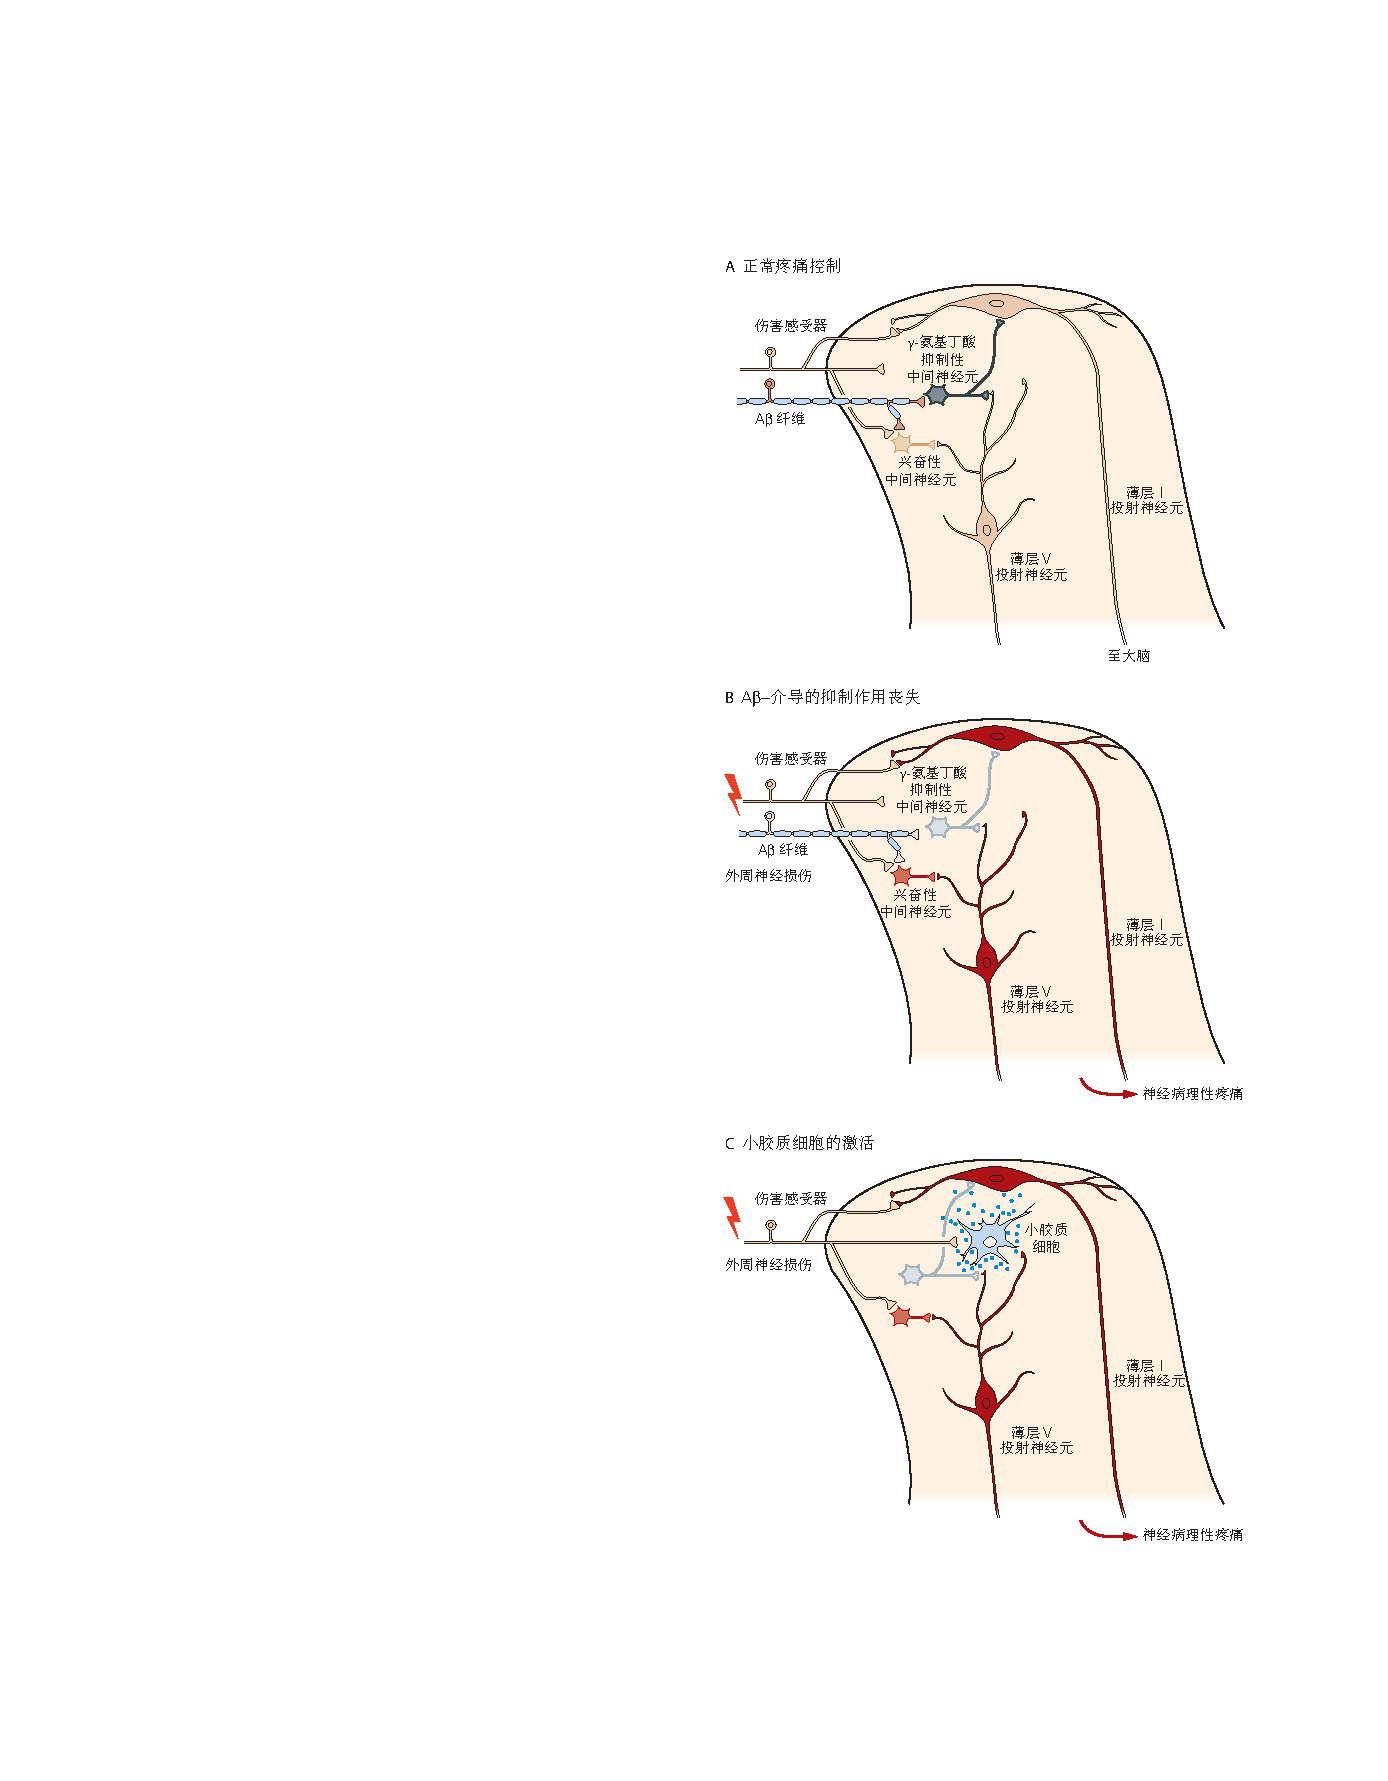
\includegraphics[width=0.5\linewidth]{chap20/fig_20_11}
	\caption{神经损伤会触发多种背角中枢致敏机制,从而导致神经性疼痛。 
		A. 在正常情况下,伤害感受器通过单突触和多突触(兴奋性)输入到 I 层和 V 层的投射神经元,将伤害感受信息传递到脑干和丘脑,从而参与背角疼痛传递回路。 (参见图 \ref{fig:20_13}。)投射神经元的输出受 GABA 能抑制性中间神经元调节,后者可被非伤害性、大直径、有髓鞘 Aβ 传入纤维激活。 
		B. 外周神经损伤可导致 Aβ 传入神经失去抑制控制,这是通过 GABA 能中间神经元的丢失、GABA 的产生减少或投射神经元对 GABA 能受体的表达减少。 
		Aβ 传入神经的病理生理发芽也可能允许非伤害性输入直接参与投射神经元(未显示),导致 Aβ 介导的机械超敏反应/异常性疼痛,这是神经性疼痛的标志。 
		C. 周围神经损伤不仅会直接激活背角神经元,还会激活小胶质细胞,小胶质细胞又会释放大量介质,增强神经元兴奋性并减少 GABA 能中间神经元施加的抑制控制。 因此,靶向小胶质细胞释放的介质为慢性疼痛的药物治疗引入了另一种潜在方法。}
	\label{fig:20_11}
\end{figure}


\section{四种主要的上行通路将伤害性信息从脊髓传递到大脑}
四种主要的上行通路——脊髓丘脑束、脊髓网状束、脊髓旁臂束和脊髓下丘脑束——为产生疼痛的中枢过程提供感觉信息。

脊髓丘脑束是脊髓中最突出的上行伤害感受通路。 
它包括位于背角 I 和 V 至 VII 层中的伤害感受特异性、热敏性和宽动态范围神经元的轴突。 
这些轴突在其起始段附近穿过脊髓中线,并在前外侧白质中上升,然后终止于丘脑核团(图 \ref{fig:20_13})。 
脊髓丘脑束在伤害性信息的传递中起着至关重要的作用。 
该束起源处的细胞通常具有离散的单侧感受野,这是我们定位疼痛刺激能力的基础。 
毫不奇怪,电刺激管道足以引起疼痛感; 相反,损伤该束(前外侧脊髓切开术),这种手术通常仅用于晚期癌症患者的顽固性疼痛,可导致损伤对侧身体一侧的痛觉明显减轻。


\begin{figure}[htbp]
	\centering
	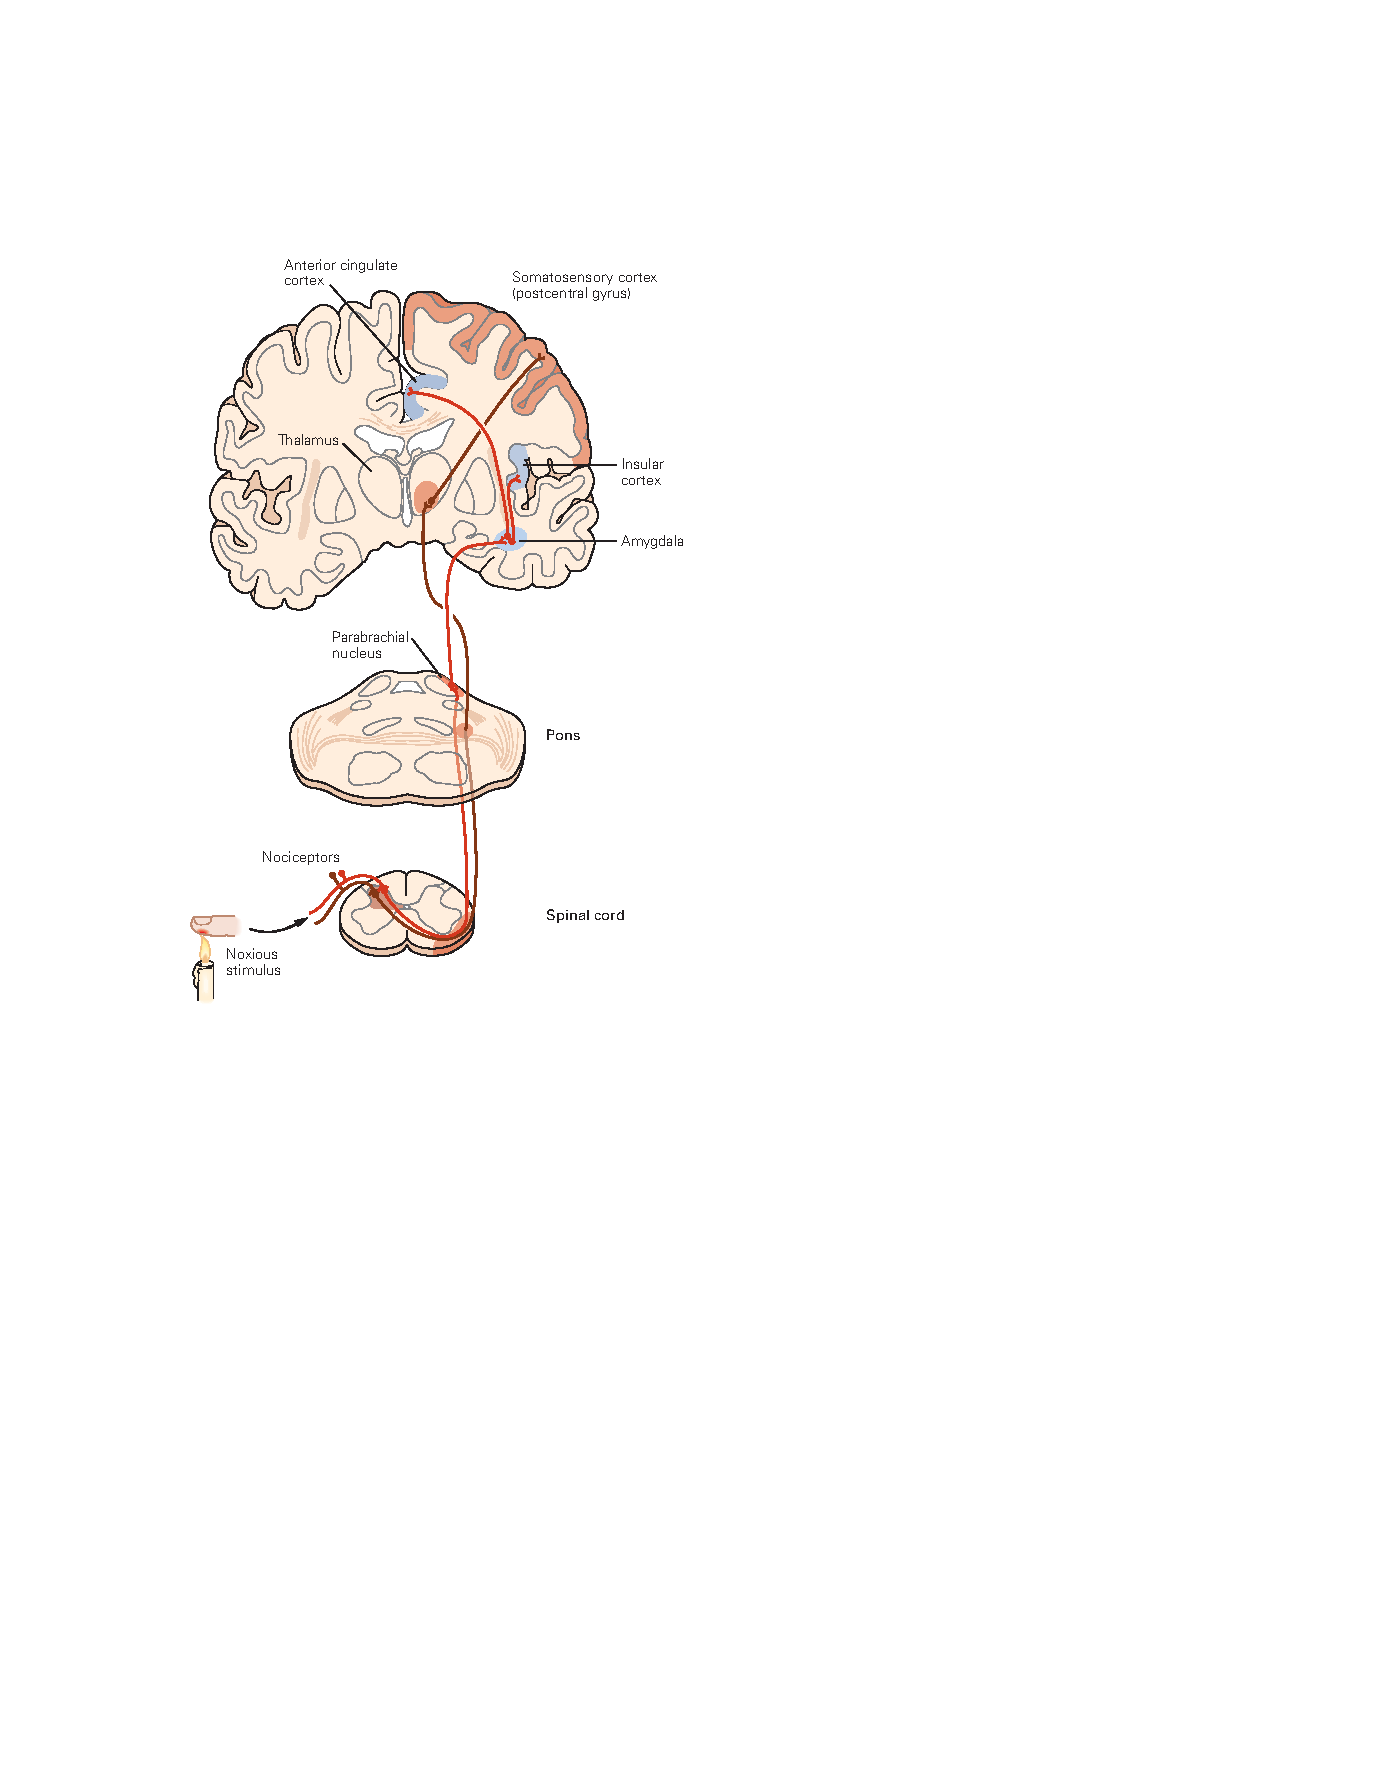
\includegraphics[width=0.7\linewidth]{chap20/fig_20_13}
	\caption{传递伤害感受信息的主要上行通路。 
		疼痛体验的感觉辨别特征通过脊髓丘脑束(棕色)从脊髓传递到腹后外侧丘脑。 
		从那里,信息主要传输到体感皮层。 
		第二条通路,(脊髓旁臂束(红色),将信息从脊髓传递到背外侧脑桥的臂旁核。
		这些神经元依次靶向边缘前脑区域,包括岛叶和前扣带皮层,它们处理情绪特征 痛苦的经历。}
	\label{fig:20_13}
\end{figure}


脊髓网状束包含椎板 VII 和 VIII 中投射神经元的轴突。 
该束在具有脊髓丘脑束轴突的脊髓前外侧象限中上升,并终止于网状结构和丘脑。 
由于脊髓网状束起源处的神经元通常具有较大的、通常是双侧的感受野,因此该通路更多地涉及弥漫性、定位不佳的疼痛的处理。


脊髓旁臂束包含 I 层和 V 层投射神经元的轴突。
沿着该束传输的信息被认为有助于疼痛的情感成分。 
该束在脊髓的前外侧象限投射到桥脑水平的臂旁核(图 \ref{fig:20_13})。 
该通路对中脑网状结构和中脑导水管周围灰质具有广泛的旁路。 
臂旁神经元投射到杏仁核,这是边缘系统的一个关键核,它调节情绪状态(第 \ref{chap:chap42} 章)。


脊髓下丘脑束包含在脊髓 I、V、VII 和 VIII 层中发现的神经元轴突。 
这些轴突投射到作为自主控制中心的下丘脑核团,参与调节伴随疼痛综合征的神经内分泌和心血管反应(第 \ref{chap:chap41} 章)。


\section{几个丘脑核将伤害性信息传递给大脑皮层}
丘脑包含几个参与伤害性信息中央处理的中继核。 
丘脑的两个最重要区域是外侧核群和内侧核群。 
外侧核群包括腹后外侧核 (VPL)、腹后内侧核 (VPM) 和后/枕核。 
VPL 和 VPM 分别通过脊髓丘脑束从背角 I 和 V 层中的伤害感受特异性神经元和宽动态范围神经元接收输入,并通过三叉神经尾核的三叉神经丘脑束接收输入,背角的三叉神经同系物 处理来自口面部区域的伤害感受信息的角。 
外侧丘脑处理有关受伤精确位置的信息,这些信息通常以急性疼痛的形式传递给意识。 
与此观点一致,外侧丘脑核中的神经元具有较小的感受野,与突触前脊髓神经元的感受野相匹配。


破坏外侧丘脑的脑血管梗塞可产生称为 Dejerine-Roussy(丘脑疼痛)综合征的中枢神经性疼痛病症。 
患有这种综合征的患者会经历自发性灼痛以及梗死对侧的异常感觉(称为感觉迟钝)。 
丘脑的电刺激也会导致剧烈疼痛。 
在一个戏剧性的临床案例中,对丘脑的电刺激重新点燃了心绞痛的感觉,这种感觉非常逼真,以至于麻醉师认为患者正在经历心脏病发作。 
这个和其他临床观察表明,在慢性神经性疼痛病症中,丘脑和皮质回路发生了根本性变化。 
这一假设与表明丘脑和体感皮层中的身体地形图不是固定的,而是会随着使用和停用而变化的研究是一致的。 
失去肢体会导致肢体的皮质表征缩小甚至消失。 
异常重组可能导致幻肢痛(图 \ref{fig:20_14})。


丘脑的内侧核群包括丘脑的内侧背核和中央外侧核以及板内复合体。 
它的主要输入来自背角 VII 和 VIII 层中的神经元。 
通往内侧丘脑的通路是哺乳动物进化中第一个明显的脊髓丘脑投射,因此被称为古脊髓丘脑束。 
它有时也被称为脊髓网状丘脑束,因为它包括通过脑干网状结构的间接连接。 
从外侧丘脑到腹后外侧核和内侧核的投射在灵长类动物中最为发达,因此被称为新脊髓丘脑束。 
内侧丘脑中的许多神经元对伤害性刺激做出最佳反应,并投射到边缘系统的许多区域,包括前扣带皮层。


\section{疼痛的感知源于皮层机制并受其控制}

\subsection{前扣带回和岛叶皮层与疼痛感知有关}
影像学研究现在表明,没有哪个皮质区域负责疼痛感知。 
相反,当一个人经历疼痛时,许多区域会被激活。 
在体感皮层中,神经元通常具有较小的感受野,并且可能不会对大多数临床综合征所特有的疼痛和疼痛的弥漫性感知做出很大贡献。 
前扣带回和岛叶皮层也包含神经元,这些神经元会被有害的体感刺激强烈和选择性地激活(方框 20-1)。


前扣带回是边缘系统的一部分,参与处理与疼痛相关的情绪状态。 
岛叶皮层接收来自丘脑和杏仁核的直接投射。 
岛叶皮层中的神经元处理有关身体内部状态的信息,并有助于疼痛反应的自主成分。 
重要的是,消融扣带皮层或从额叶皮层到扣带皮层的通路的神经外科手术可减少疼痛的情感特征,同时不会消除识别损伤强度和位置的能力。 
患有岛叶皮层病变的患者表现出明显的疼痛无症状综合征。 
他们认为伤害性刺激是痛苦的,可以区分剧烈疼痛和钝痛,但无法表现出适当的情绪反应。 
这些观察表明,岛叶皮层是一个整合了疼痛的感觉、情感和认知成分的区域。


\subsection{痛觉受伤害性和非伤害性传入纤维活动平衡的调节}
脊髓背角的许多投射神经元选择性地对有害输入做出反应,但其他投射神经元接收来自伤害性传入神经和非伤害性传入神经的会聚输入。 
将感觉输入汇聚到脊柱投射神经元上调节疼痛处理的概念最早出现于 1960 年代。


Ronald Melzack 和 Patrick Wall 提出,伤害性传入神经和非伤害性传入神经活动的相对平衡可能会影响疼痛的传递和感知。 
特别是,他们提出通过激活背角的抑制性中间神经元来激活非伤害性感觉神经元,从而关闭伤害性信号传入传递的“门”,而伤害性感觉神经元的激活可以打开该“门”。 
在这个门控理论的原始和最简单的形式中,大纤维和小纤维之间的相互作用发生在脊髓背角投射神经元的第一个可能会聚点(图 \ref{fig:20_16})。 
我们现在知道,这种相互作用也可以发生在许多脊髓上中继中心。

\begin{figure}[htbp]
	\centering
	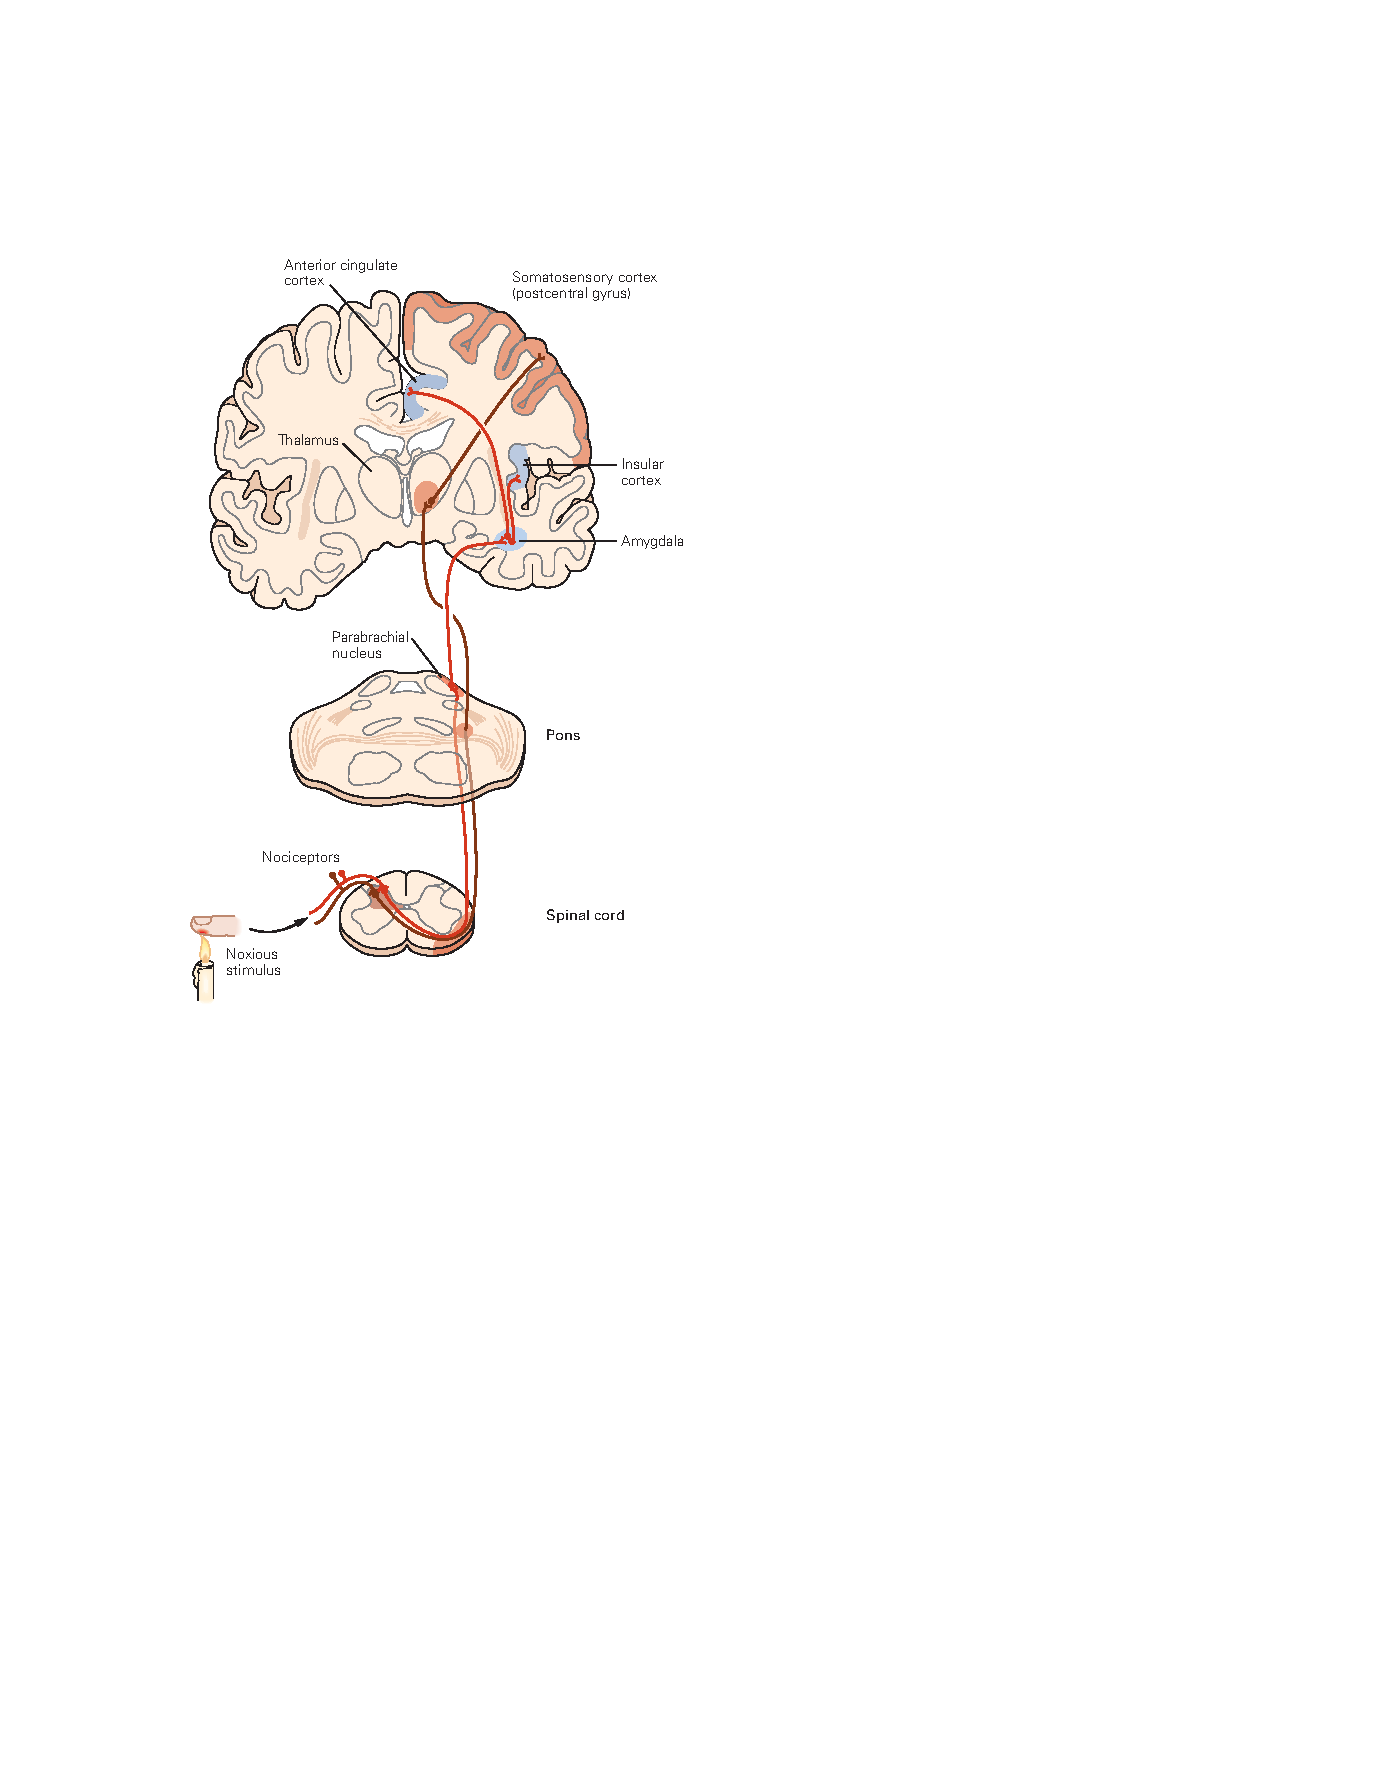
\includegraphics[width=0.7\linewidth]{chap20/fig_20_13}
	\caption{疼痛的闸门控制理论。 
		门控假说在 1960 年代提出,以解释低阈值初级传入纤维的激活可以减轻疼痛这一事实。 该假设侧重于脊髓背角神经元的相互作用:伤害性 (C) 和非伤害性 (Aa) 感觉神经元、投射神经元和抑制性中间神经元。 
		在模型的原始版本中,如图所示,投射神经元被两类感觉神经元兴奋,并被浅表背角中的中间神经元抑制。 
		这两类感觉纤维也终止于抑制性中间神经元; C 纤维间接抑制中间神经元,从而增加投射神经元的活动(从而“打开门”),而 Aβ 纤维刺激中间神经元,从而抑制投射神经元的输出(并“关闭门”)。}
	\label{fig:20_16}
\end{figure}

不同感觉方式的融合概念为设计新的疼痛疗法提供了重要基础。 
从最广泛的意义上看,脊柱或脊柱上部位的高阈值和低阈值输入的融合为关于疼痛感知的几项经验观察提供了合理的解释。 
手被锤击或烧伤后的抖动是一种反射行为,可以通过激活抑制有害刺激信息传递的大直径传入纤维来减轻疼痛。


融合的想法也有助于促进使用经皮神经电刺激 (TENS) 和脊髓刺激来缓解疼痛。 
使用 TENS,放置在外围位置的刺激电极会激活大直径传入纤维,这些纤维支配重叠区域,但也围绕受伤和疼痛区域。 
疼痛减轻的身体区域映射到脊髓的那些区段,来自该身体区域的伤害感受和非伤害感受传入终止。 
这符合直觉:您不会通过摇动左腿来减轻右臂的疼痛。


\subsection{大脑的电刺激产生镇痛}
几个内源性疼痛调节位点位于大脑中。 
抑制伤害感受的一种有效方法包括刺激导水管周围灰色区域,即围绕第三脑室和大脑导水管的中脑区域。 
在实验动物中,刺激该区域会引起深度和选择性镇痛。 
这种刺激产生的镇痛作用具有显着的特异性; 动物仍然会对对疼痛不敏感的身体区域的触摸、压力和温度做出反应。 
刺激诱发镇痛已被证明是在有限数量的人类疼痛条件下缓解疼痛的有效方法。


刺激导水管周围灰质会阻断通常由有害刺激引起的脊髓介导的退缩反射。 
导水管周围灰质中的神经元很少直接投射到脊髓的背角。 
大多数与延髓前腹侧神经元建立兴奋性联系,包括中线区域称为中缝大核的血清素能神经元。 
这些血清素能神经元的轴突通过外侧索的背侧区域投射到脊髓,在那里它们与背角 I、II 和 V 层中的神经元形成抑制性连接(图 \ref{fig:20_17})。 
因此,刺激延髓前腹侧会抑制许多类背角神经元的放电,包括向大脑传递传入伤害性信号的主要上行通路的投射神经元。

\begin{figure}[htbp]
	\centering
	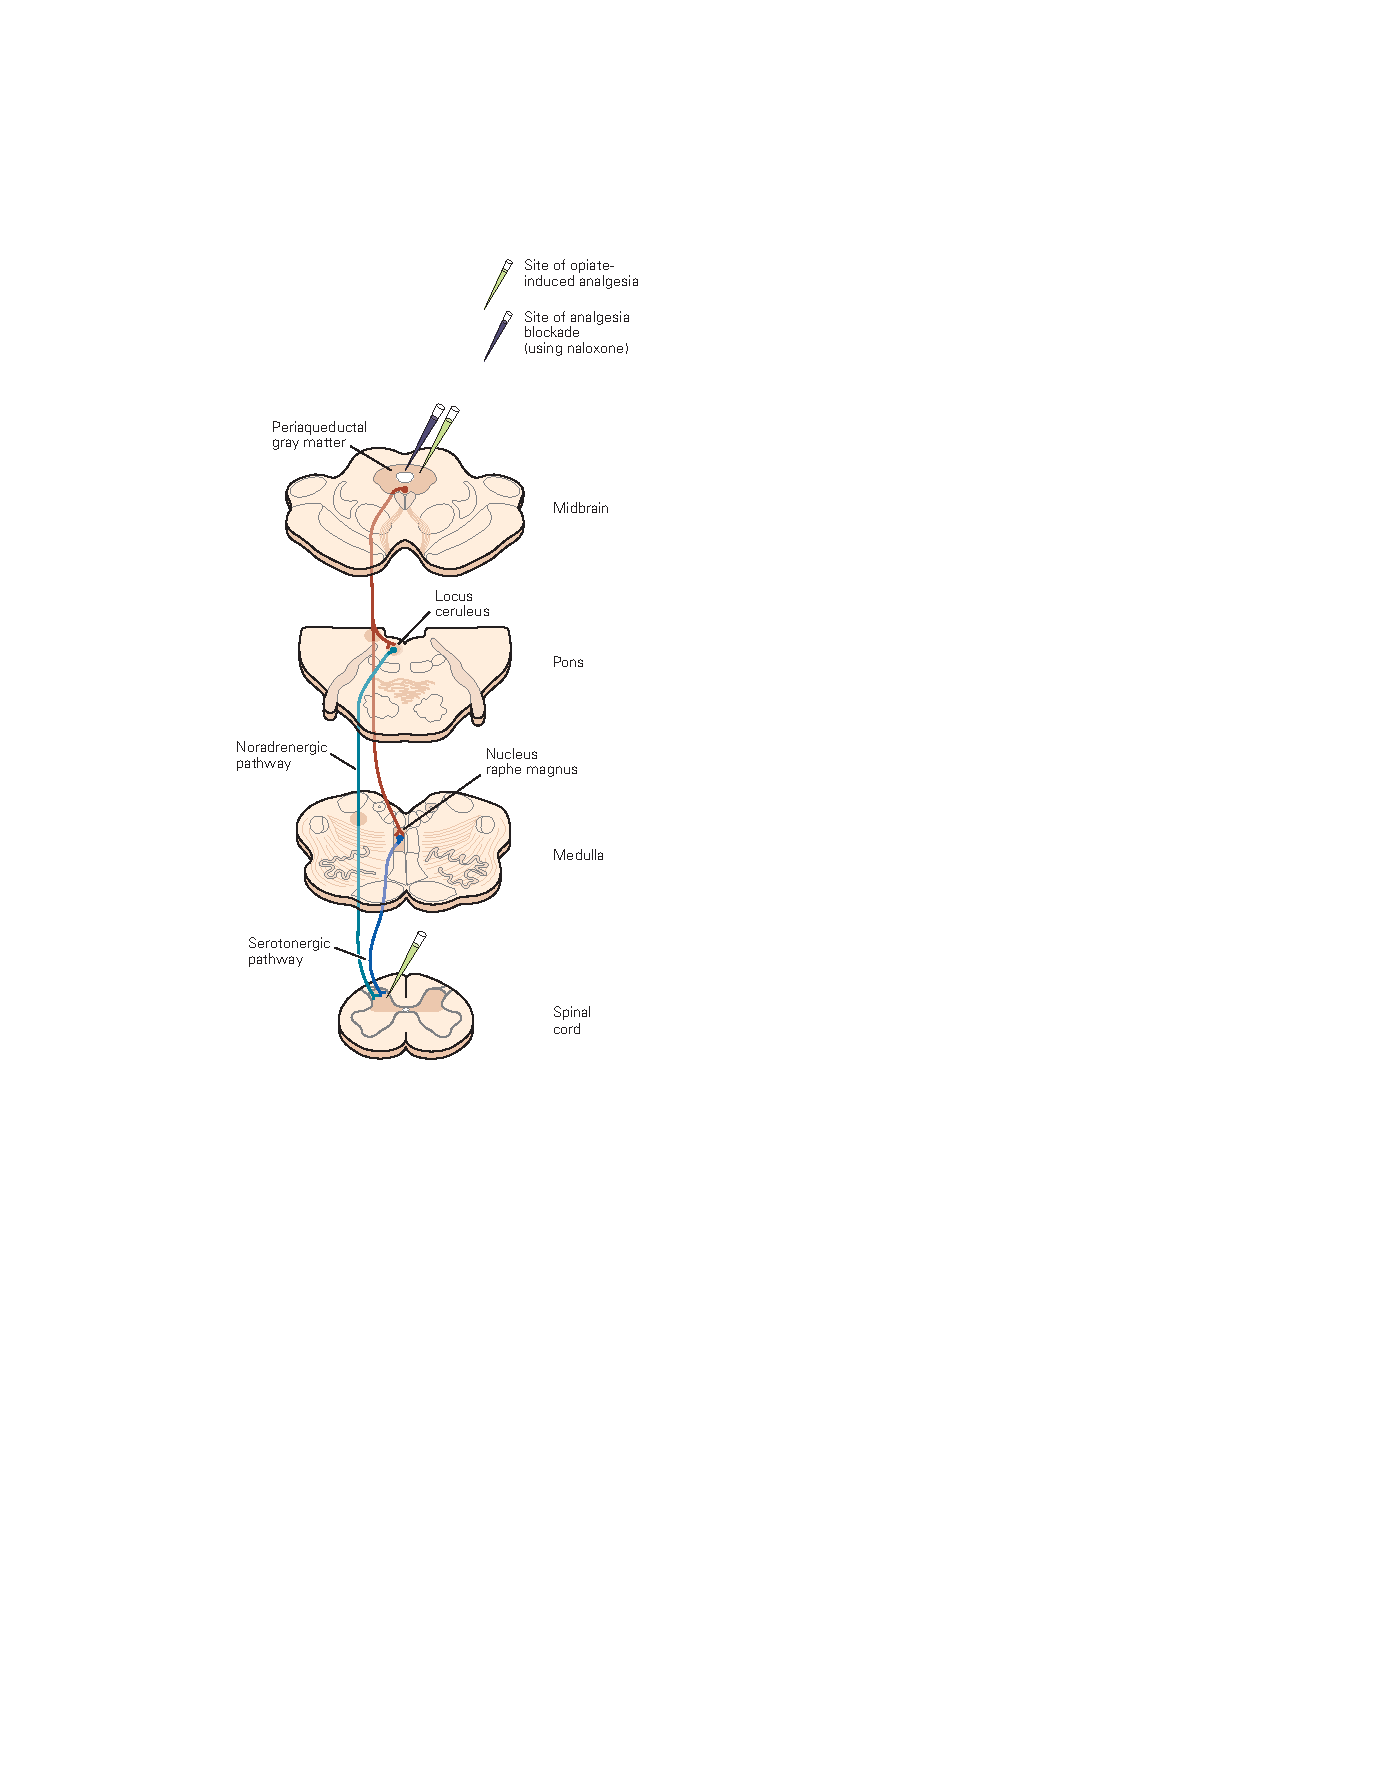
\includegraphics[width=0.7\linewidth]{chap20/fig_20_17}
	\caption{下行单胺能通路调节脊髓中的伤害性中继神经元。 
		5-羟色胺能途径出现在中缝大核中,并通过背外侧索投射到脊髓的背角。 
		去甲肾上腺素能系统出现在脑桥和延髓的蓝斑和其他核团中。 (有关单胺能神经元的位置和投射,请参见图 40-11A。)在脊髓中,这些下行通路通过直接连接以及通过背角表层的中间神经元抑制伤害性投射神经元。 
		5-羟色胺能中缝大核和去甲肾上腺素能核都接收来自导水管周围灰色区域神经元的输入。 
		显示了阿片样肽表达的位点和外源性阿片样物质的作用。}
	\label{fig:20_17}
\end{figure}

第二个主要的单胺能下行系统也可以抑制背角伤害感受神经元的活动。 这种去甲肾上腺素能系统起源于蓝斑和延髓和脑桥的其他核团(图 \ref{fig:20_17})。 
通过直接和间接的突触作用,这些投射抑制了背角 I 和 V 层中的神经元。


\section{阿片肽有助于内源性疼痛控制}
自公元前 3300 年苏美尔人发现罂粟以来,该植物的活性成分,如吗啡和可待因等阿片类药物,已被公认为强效镇痛剂。 
在过去的二十年里,我们已经开始了解许多阿片类药物发挥镇痛作用的分子机制和神经回路。 
此外,我们已经认识到,参与刺激产生的镇痛和阿片类镇痛的神经网络密切相关。


两个关键发现导致了这些进步。 
首先是认识到吗啡和其他阿片类药物与脊髓和大脑神经元上的特定受体相互作用。 
第二个是分离在这些受体上具有类鸦片活性的内源性神经肽。 
阿片拮抗剂纳洛酮阻断刺激产生的镇痛作用的观察结果提供了大脑含有内源性阿片样物质的第一个线索。


\subsection{内源性阿片肽及其受体分布在疼痛调节系统中}
阿片受体分为四大类:mu (μ)、delta (δ)、kappa (κ) 和孤啡肽 FQ。 
编码每一种受体类型的基因构成了 G 蛋白偶联受体的一个亚家族。 
μ受体特别多样化; 已经鉴定出许多 μ 受体亚型,其中许多具有不同的表达模式。 
这一发现促使人们寻找针对特定亚型的镇痛药。


阿片受体最初是根据不同激动剂化合物的结合亲和力定义的。 
吗啡和其他阿片类生物碱是 μ 受体的有效激动剂,镇痛剂的效力与其与 μ 受体结合的亲和力之间存在紧密相关性。 
μ 受体基因失活的小鼠对吗啡和其他阿片类激动剂不敏感。 
许多阿片类拮抗剂药物,如纳洛酮,也与 μ 受体结合并与吗啡竞争受体占用而不激活受体信号传导。


μ 受体高度集中在脊髓浅表背角、腹侧髓质和导水管周围灰质——调节疼痛的重要解剖部位。 
然而,与其他类别的阿片受体一样,它们也存在于中枢和周围神经系统的许多其他部位。 
它们的广泛分布解释了为什么全身给药的吗啡会影响除疼痛感知之外的许多生理过程。


阿片受体的发现及其在中枢和外周神经系统中神经元的表达导致了四大类内源性阿片肽的定义,每一种都与一类特定的阿片受体相互作用(表 20-1)。


三个类别——脑啡肽、β-内啡肽和强啡肽——具有最好的特征。 
这些阿片肽由大的多肽前体通过酶促裂解形成(图 \ref{fig:20_18}),并由不同的基因编码。 
尽管氨基酸序列不同,但每个都包含 Tyr-Gly-Gly-Phe 序列。 
β-内啡肽是一种前体的裂解产物,它也能产生活性肽促肾上腺皮质激素 (ACTH)。 
β-内啡肽和促肾上腺皮质激素均由垂体细胞合成,并在应激反应下释放到血液中。 
强啡肽来源于强啡肽基因的多蛋白产物。

\begin{figure}[htbp]
	\centering
	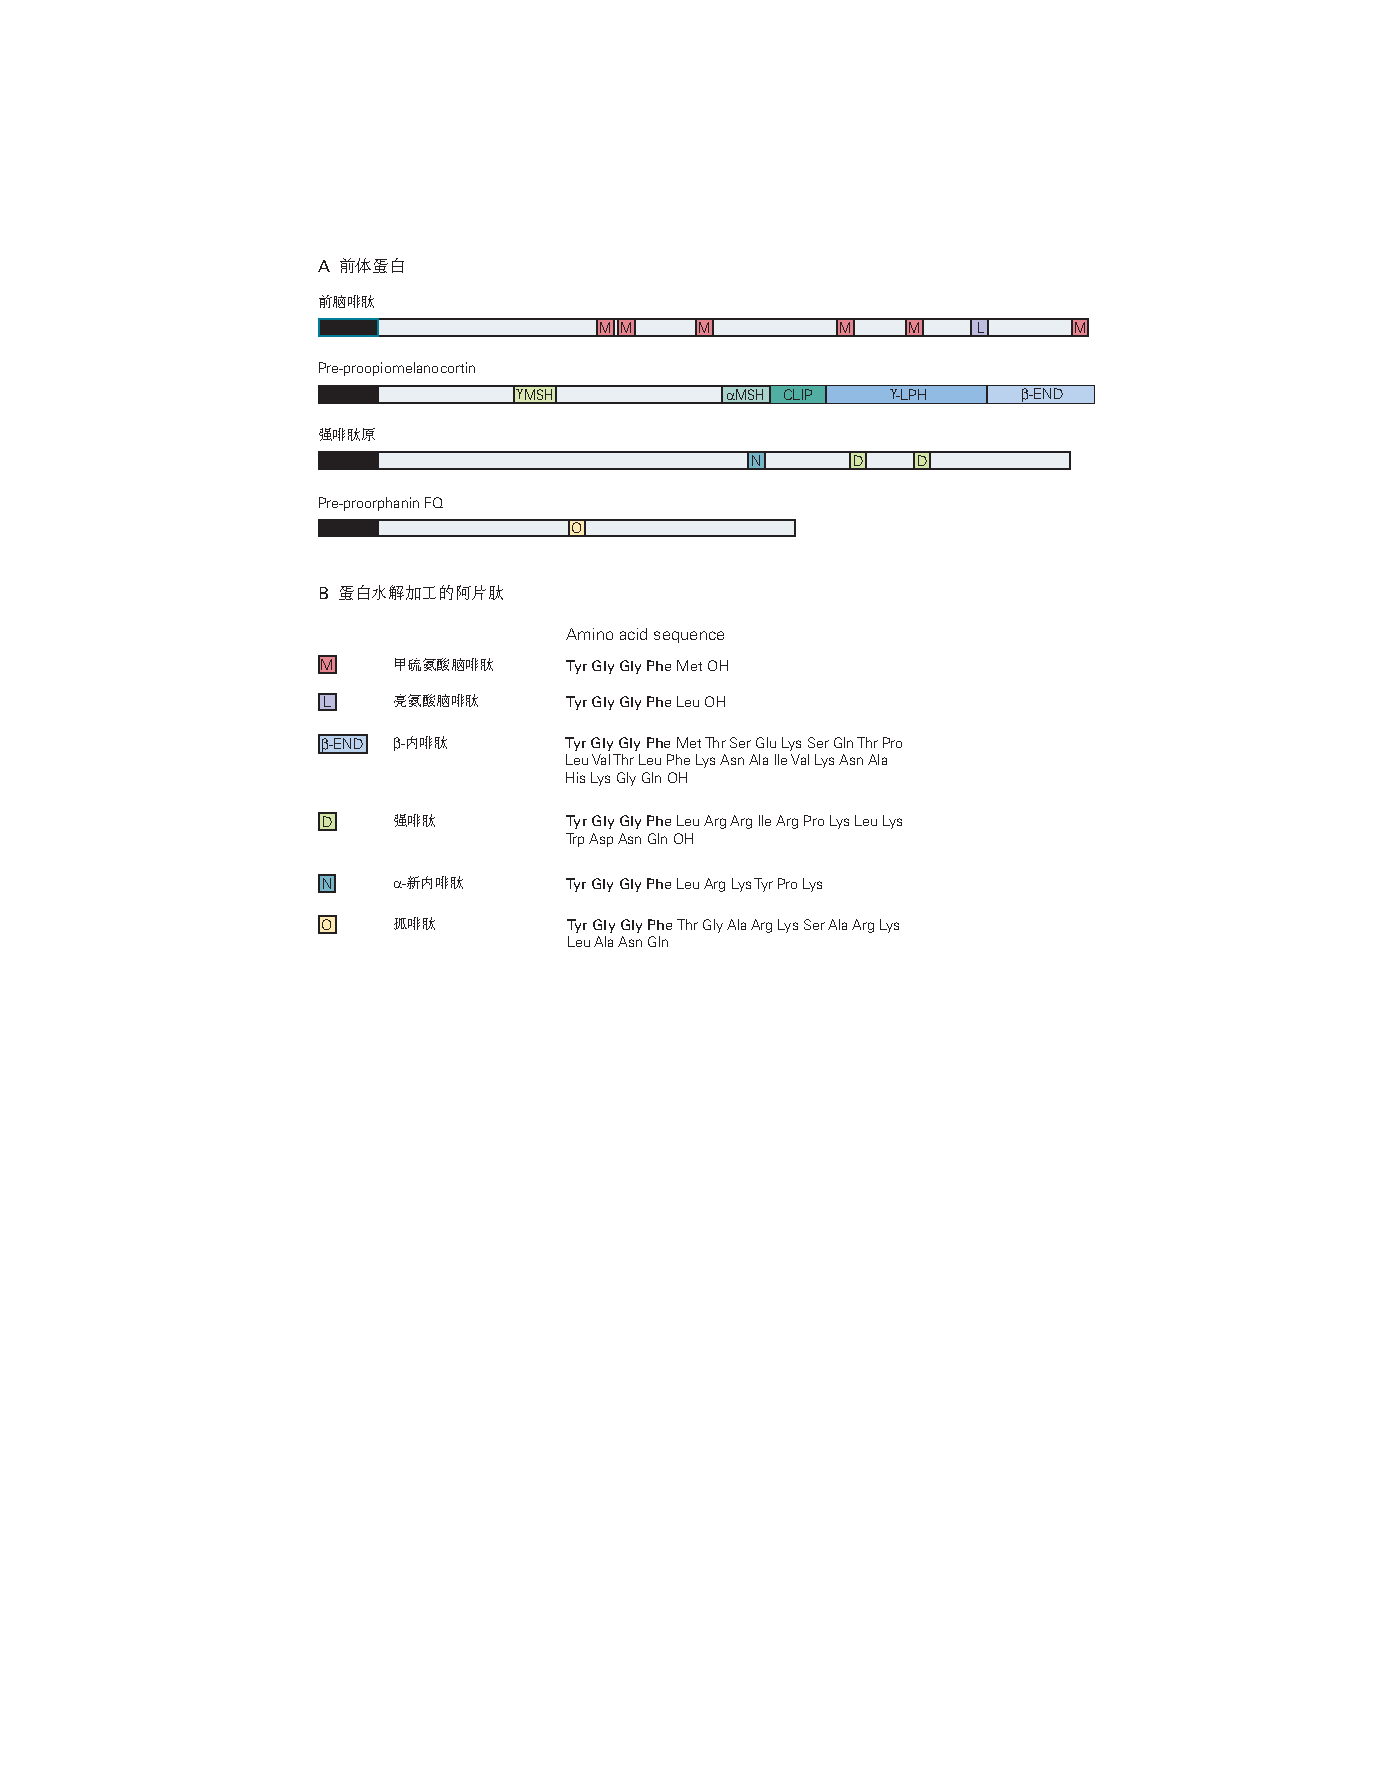
\includegraphics[width=1.0\linewidth]{chap20/fig_20_18}
	\caption{四个内源性阿片肽家族来自大的前体多蛋白。 
		A. 蛋白水解酶切割每个前体蛋白以生成较短的生物活性肽,其中一些显示在该图中。 
		脑啡肽原前体蛋白包含多个拷贝的甲硫氨酸-脑啡肽 (M)、亮氨酸-脑啡肽 (L) 和几种扩展的脑啡肽。 
		原阿黑皮素(POMC)含有β-内啡肽(β-END、促黑素细胞激素(MSH)、促肾上腺皮质激素(ACTH)和促肾上腺皮质激素样中叶肽(CLIP)。
		强啡肽原前体可产生强啡肽(D)和α -neoendorphin (N). pro-orphanin precursor contains the orphanin FQ peptide (O), also called nociceptin. 黑色域表示信号肽。
		B. 蛋白水解加工的生物活性肽的氨基酸序列。氨基酸残基以粗体显示 类型介导与阿片受体的相互作用。(经许可改编自 Fields 1987。)}
	\label{fig:20_18}
\end{figure}

四类阿片肽的成员广泛分布在中枢神经系统中,各个肽位于与伤害性信息的处理或调节相关的位点。 
含有脑啡肽和强啡肽的神经元细胞体和轴突末端存在于脊髓的背角,特别是 I 和 II 层,以及延髓头端腹侧和导水管周围灰质中。 
合成 β-内啡肽的神经元主要局限于下丘脑; 它们的轴突终止于导水管周围灰色区域和脑干中的去甲肾上腺素能神经元。 
孤儿素 FQ 似乎参与广泛的其他生理功能。


\subsection{吗啡通过激活阿片受体来控制疼痛}
将低剂量的吗啡、其他阿片类药物或阿片肽直接显微注射到大鼠大脑的特定区域会产生强大的镇痛作用。 
导水管周围灰色区域是最敏感的部位之一,但将吗啡局部给药到其他区域,包括脊髓,也会产生强大的镇痛作用。


可通过将阿片拮抗剂纳洛酮注射到导水管周围灰质区域或中缝大核中来阻断吗啡诱导的全身镇痛(图 \ref{fig:20_17})。 
此外,脊髓背外侧索的双侧横切可阻断中枢给药吗啡诱导的镇痛作用。 
因此,吗啡的中枢镇痛作用涉及到脊髓下行通路的激活,与介导脑电刺激和吗啡产生的镇痛作用的下行通路相同。


与其他地方一样,在脊髓中,吗啡通过模仿内源性阿片肽的作用发挥作用。 
脊髓浅背角包含表达脑啡肽和强啡肽的中间神经元,这些神经元的末端靠近伤害性感觉神经元和脊髓投射神经元形成的突触(图 \ref{fig:20_19} A)。 
此外,μ、δ 和 κ 受体位于伤害性感觉神经元的末端以及接收传入伤害性输入的背角神经元的树突上,因此将内源性阿片肽置于调节感觉输入的战略位置。 
介导缓慢持续性疼痛或“第二次疼痛”的 C 纤维伤害感受器比介导快速和急性疼痛或“第一次疼痛”的 Aδ 伤害感受器具有更多的 μ 受体(图 \ref{fig:20_1})。 
这可能有助于解释为什么吗啡在治疗持续性疼痛而不是急性疼痛方面更有效。

\begin{figure}[htbp]
	\centering
	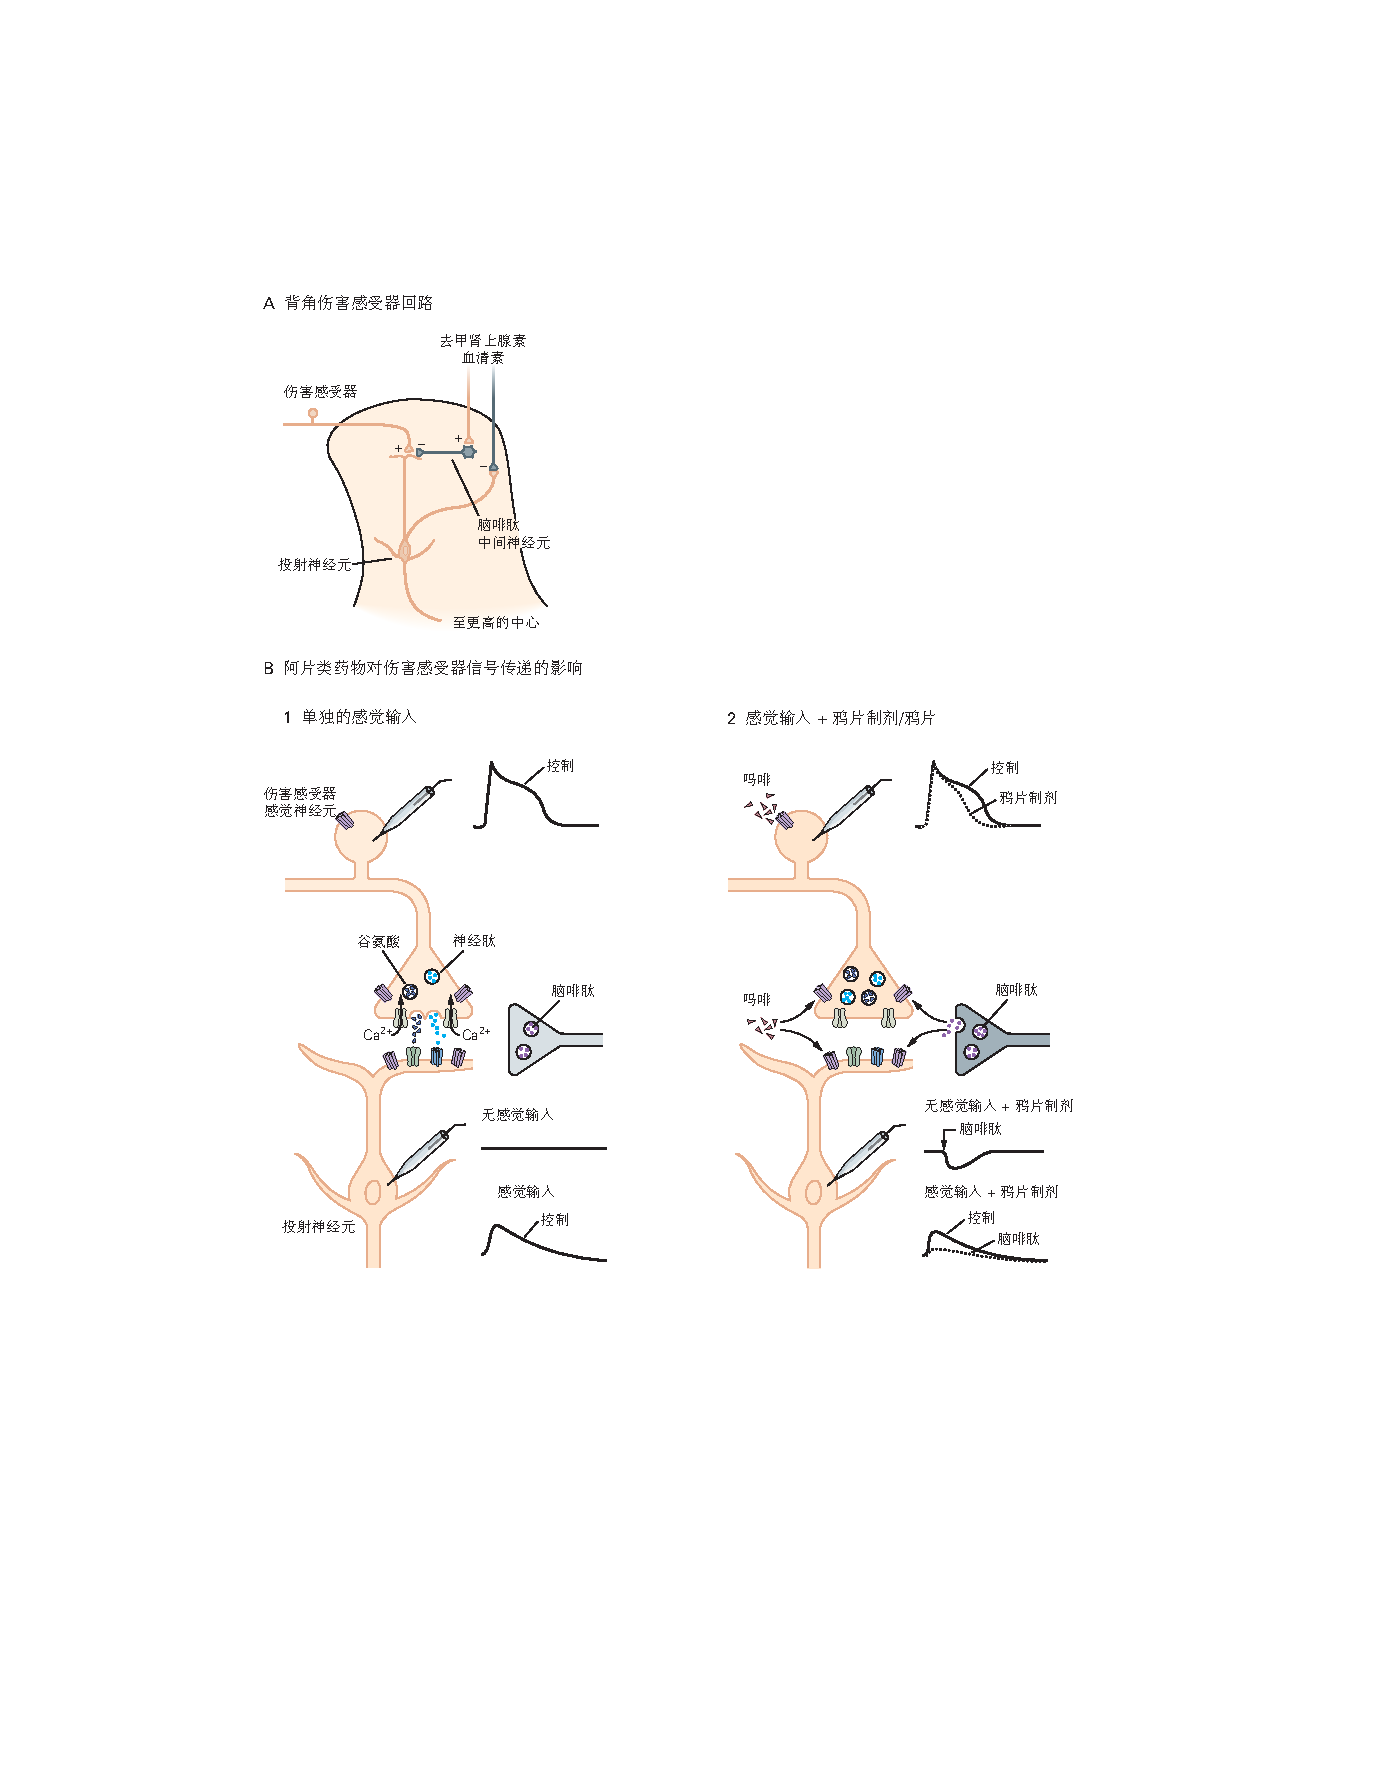
\includegraphics[width=1.0\linewidth]{chap20/fig_20_19}
	\caption{脊髓中的局部中间神经元整合了下行和传入伤害性通路。 
		A. 伤害性传入纤维、局部中间神经元和下行纤维在脊髓的背角相互连接(另请参见图 20-3B)。 
		伤害性纤维终止于二阶投射神经元。 
		局部 GABAergic 和含脑啡肽的抑制性中间神经元在这些突触处发挥突触前和突触后抑制作用。 
		脑干中的血清素能和去甲肾上腺素能神经元激活局部中间神经元并抑制投射神经元的活动。 
		失去这些抑制控制会导致持续的疼痛和疼痛超敏反应。 
		B. 背角突触伤害性信号的调节。 
		1. 伤害感受器的激活导致初级感觉神经元释放谷氨酸和神经肽,从而在投射神经元中产生兴奋性突触后电位。 
		2. 阿片类药物减少突触后电位的持续时间,可能是通过减少 Ca2+ 流入,从而减少从初级感觉终端释放递质。 
		此外,阿片类药物通过激活 K+ 电导使背角神经元超极化,从而降低背角神经元突触后电位的振幅。}
	\label{fig:20_19}
\end{figure}


阿片类药物(阿片类药物和阿片类肽)通过两种主要机制调节背角突触处的伤害感受传递。 
首先,它们增加了背角神经元的膜 K+ 电导,使神经元超极化并增加了它们的激活阈值。 
其次,通过与突触前感觉神经末梢上的受体结合,阿片类药物阻断电压门控 Ca2+ 通道,从而减少 Ca+ 进入感觉神经末梢(图 \ref{fig:20_19} B)。 
这种作用反过来会抑制神经递质的释放,从而减少突触后背角神经元的激活。


阿片受体在大脑和外周的广泛分布是阿片类药物产生的许多副作用的原因。 
由肠和肛门括约肌的肌肉表达的阿片受体的激活导致便秘。 
同样,阿片受体介导的孤束核神经元活动抑制是呼吸抑制和心血管副作用的基础。 
出于这个原因,阿片类药物的直接脊髓给药具有显着的优势。 
注入脊髓蛛网膜下腔的脑脊液中的吗啡与背角中的阿片受体相互作用,引起深度和长时间的镇痛。 
吗啡的脊柱给药现在常用于治疗术后疼痛,尤其是分娩时与剖宫产相关的疼痛。 
除了产生延长的镇痛作用外,鞘内注射吗啡的副作用较少,因为药物不会扩散到远离注射部位的地方。 
向脊髓连续局部输注吗啡也已用于治疗某些癌症疼痛。


阿片类药物还作用于大脑皮层的受体。 
例如,有证据表明阿片类药物可以通过前扣带回的作用影响疼痛体验的情感成分。 
最有趣的是,有相当多的证据表明安慰剂镇痛涉及内啡肽释放,并且可以被纳洛酮逆转。 
这一发现强调,对安慰剂的反应并不表明疼痛是某种想象出来的。 
此外,安慰剂镇痛是任何止痛药(包括吗啡)整体镇痛作用的组成部分,前提是患者认为治疗有效。 
另一方面,其他一些减轻疼痛的心理干预,即催眠,似乎并不涉及内啡肽的释放。


\subsection{对阿片类药物的耐受和依赖是截然不同的现象}
长期使用吗啡会引发重大问题,最显着的是耐受性和心理依赖性(成瘾)(第 \ref{chap:chap43} 章)。 
重复使用吗啡来缓解疼痛会导致患者对药物的镇痛作用产生抵抗力,因此需要逐渐增加药物剂量才能达到相同的治疗效果。 
一种理论认为,耐受性是阿片受体与其 G 蛋白转导物解偶联的结果。 
然而,由于纳洛酮与 μ-阿片受体的结合可以在耐受受试者中引发戒断症状,因此阿片受体似乎在耐受状态下仍然活跃。 
因此,耐受性也可能反映了细胞对阿片受体激活的反应,这种反应抵消了阿片剂的作用并重置了系统。 
随之而来的是,当阿片类药物突然被移除或纳洛酮被给药时,这种补偿反应就会暴露出来,从而导致戒断反应。


这种生理耐受性与依赖/成瘾不同,依赖/成瘾是一种对药物的心理渴望,与药物滥用有关,并导致阿片类药物使用障碍。 
鉴于与阿片类药物相关的死亡人数惊人地增加,无论是由于处方阿片类药物的滥用和过量服用还是由于一系列社会经济因素,进一步研究有助于发展和区分耐受性和成瘾的机制是必不可少的。 
毫无疑问,吗啡和其他阿片类药物在控制术后疼痛方面非常有用。 
它们是否对非癌症患者的慢性疼痛管理同样有效仍存在争议,需要进一步研究。


\section{亮点}

1. 外周伤害性轴突,细胞体位于背根神经节,包括小直径无髓鞘 (C) 和有髓鞘 (Aδ) 传入神经。 
较大直径的 Aβ 传入神经仅对无害刺激有反应,但在受伤后可激活中枢神经系统疼痛回路。 


2. 所有伤害感受器都使用谷氨酸作为兴奋性神经递质; 许多还表达兴奋性神经肽协同递质,例如 P 物质或 CGRP。 

3. 伤害感受器还通过它们对温度、植物产品、机械刺激或 ATP 敏感的不同受体的表达进行分子区分。 
由于许多这些分子,包括电压门控 Na+ 通道的 Nav1.7 亚型,仅在感觉神经元中表达,因此它们的选择性药理学靶向暗示了一种镇痛药物开发的新方法。 


4. 伤害感受器终止于脊髓的背角,在那里它们激发中间神经元和投射神经元。 
神经肽也从伤害感受器的外周末端释放,并导致神经源性炎症,包括外周血管的血管扩张和外渗。 
开发 CGRP 抗体以阻断血管舒张是治疗偏头痛的新方法。 


5. 背角投射神经元的主要大脑目标是腹后外侧丘脑,它处理疼痛刺激的位置和强度特征。 
其他神经元靶向背外侧脑桥的臂旁核 (PB)。 
反过来,PB 神经元投射到大脑的边缘区域,该区域处理疼痛体验的情感/情绪特征。
 

6. 异常性疼痛,由无害刺激产生的疼痛,部分是由于伤害感受器的外周敏化引起的。 
当存在组织损伤和炎症时会发生外周致敏,并涉及对 NSAID 敏感的前列腺素的产生,从而降低激活伤害感受器的阈值。 
NSAIDs 的一大优势是它们作用于外周,说明了努力开发药物疗法的重要性,例如 NGF 抗体,它不能穿过血脑屏障,从而减少它们在中枢神经系统中产生不良副作用的可能性 系统。 


7. 痛觉过敏(对疼痛刺激的反应加剧疼痛)和异常性疼痛也由背角活动改变引起——这是一种中枢敏化过程,有助于疼痛传递神经元的自发活动和伤害感受信号的放大。 
脊髓 NMDA 受体的谷氨酸激活以及小胶质细胞和星形胶质细胞的激活尤其有助于周围神经损伤后可能发生的神经性疼痛。 
了解中枢敏化的后果对于防止从急性疼痛转变为慢性疼痛至关重要。 


8. 在正常情况下,大直径非伤害性传入神经的输入可以通过在背角接合 GABA 能抑制回路来减少伤害性信息向大脑的传输。 
这种抑制控制是振动和经皮电刺激产生的疼痛缓解的基础。 
然而,当损伤诱导中枢敏化时,Aβ 输入介导机械异常性疼痛。
 

9. 阿片类药物是治疗剧烈疼痛最有效的药理工具。 
阿片类药物和相关内源性阿片肽的抑制作用是由神经递质释放减少或突触后神经元超极化引起的。 
阿片受体拮抗剂纳洛酮可以阻断所有阿片样物质的作用。 


10. 内源性阿片类药物,包括脑啡肽和强啡肽,及其阿片类药物受体靶点不仅仅在大脑的疼痛相关区域表达。
因此,阿片类药物的全身给药与许多不良副作用有关,包括便秘、呼吸抑制和奖赏系统激活。 
后者可能导致心理依赖和最终滥用。
许多这些不良副作用限制了阿片类药物用于长期疼痛控制的使用。


11. 大脑不仅接收导致疼痛感知的伤害感受信息,而且还通过内啡肽介导的疼痛控制系统调节脊髓的输出以减轻疼痛。 
中脑导水管周围灰质的电刺激可以激活下行抑制控制系统,可能涉及内啡肽,从而减少疼痛信息从脊髓传递到大脑。


12. 一些心理操作(例如,安慰剂镇痛)产生的疼痛缓解涉及内啡肽释放;
其他操作,例如催眠,则不会。


13. 长期使用阿片类药物会产生耐受性和心理依赖性。 
耐受性表现为需要更高剂量的阿片剂才能达到相同的生理终点。 
相比之下,心理依赖涉及大脑奖励系统的激活和可能导致滥用的渴望的发展。


\section{选读}
\section{参考文献}